\documentclass[11pt, a4paper]{article} %tamaño mínimo de letra 11pto.

\usepackage{graphicx} 
\usepackage{listings} 
\usepackage{multicol}
\usepackage{siunitx} 
\usepackage{caption} 
\usepackage{hyperref} 
\usepackage{amsmath} 
\usepackage[bottom]{footmisc}
\graphicspath{ {./images/} }
\usepackage[spanish]{babel} %Español 
\usepackage[utf8]{inputenc} %Para poder poner tildes
\usepackage{vmargin} %Para modificar los márgenes
\usepackage{float} 
\setmargins{2.5cm}{1.5cm}{16.5cm}{23.42cm}{10pt}{1cm}{0pt}{2cm}
%margen izquierdo, superior, anchura del texto, altura del texto, altura de los encabezados, espacio entre el texto y los encabezados, altura del pie de página, espacio entre el texto y el pie de página
\captionsetup{textfont=it}
\sisetup{binary-units=true}
\lstset{breaklines=true, basicstyle=\ttfamily\small,
keywordstyle=\color{red}, % Color for keywords
    commentstyle=\color{blue}, % Color for comments
    }

\begin{document}
%%%%%%Portada%%%%%%%
\begin{titlepage}
\centering
{ \bfseries \Large UNIVERSIDAD COMPLUTENSE DE MADRID}
\vspace{0.5cm}

{\bfseries  \Large FACULTAD DE CIENCIAS FÍSICAS} 
\vspace{1cm}

{\large DEPARTAMENTO DE ESTRUCTURA DE LA MATERIA, FÍSICA TÉRMICA Y ELECTRÓNICA}
\vspace{0.8cm}

%%%%Logo Complutense%%%%%
{
\includegraphics[width=0.35\textwidth]{logo_UCM}}

%%Para ajustar la portada a una sola página se puede reducir el tamaño del logo
\vspace{0.8cm}

%%PORTADA

{\bfseries \Large TRABAJO DE FIN DE GRADO}
\vspace{2cm}

{\Large Código de TFG:  [C\'odigo TFG] } \vspace{5mm}

{\Large Sistema de comunicaciones inalámbricas}\vspace{5mm}

{\Large Wireless communication system}\vspace{5mm}

{\Large Supervisor/es: Javier Olea Ariza}\vspace{20mm} 

{\bfseries \LARGE Jose Luis Gutiérrez Moreno}\vspace{5mm} 

{\large Grado en Ingeniería Electrónica de Comunicaciones}\vspace{5mm} 

{\large Curso acad\'emico 2023-2024}\vspace{5mm} 

{\large Convocatoria XXXX}\vspace{5mm} 

\end{titlepage}

%% AGRADECIMIENTOS
% \newpage
%    A los chavales, por habernos acompañado y haber sufrido juntos a lo largo de estos años; a mis amigos, Fernando, Alejandro, Pablo, Dani, Rafa, César, Irene P, Irene C, Natalia, Ichi, Marta, Celia, Rubén, Alba, Viti, Miguel, Laura, Jesús, Javo, Marta, Enchufe, Rojas, Lim\'on y los xd hermanos,  mi via escape y apoyo a lo largo de mi vida.
\paragraph{}
En especial a Marti, mi apoyo incondicional y redactora personal; a mi hermano, por estar siempre juntos y porque triunfe en sus oposiciones; a Mario, por aportar la realidad y la ayuda en la práctica; a mi madre y a mi tio, porque siempre han confiado en mí y me han guiado hasta lo que soy hoy. Y sobretodo, a la yaya, mi pilar fundamental y la mayor fan que se puede tener.
\begin{figure}[h]
    \centering
    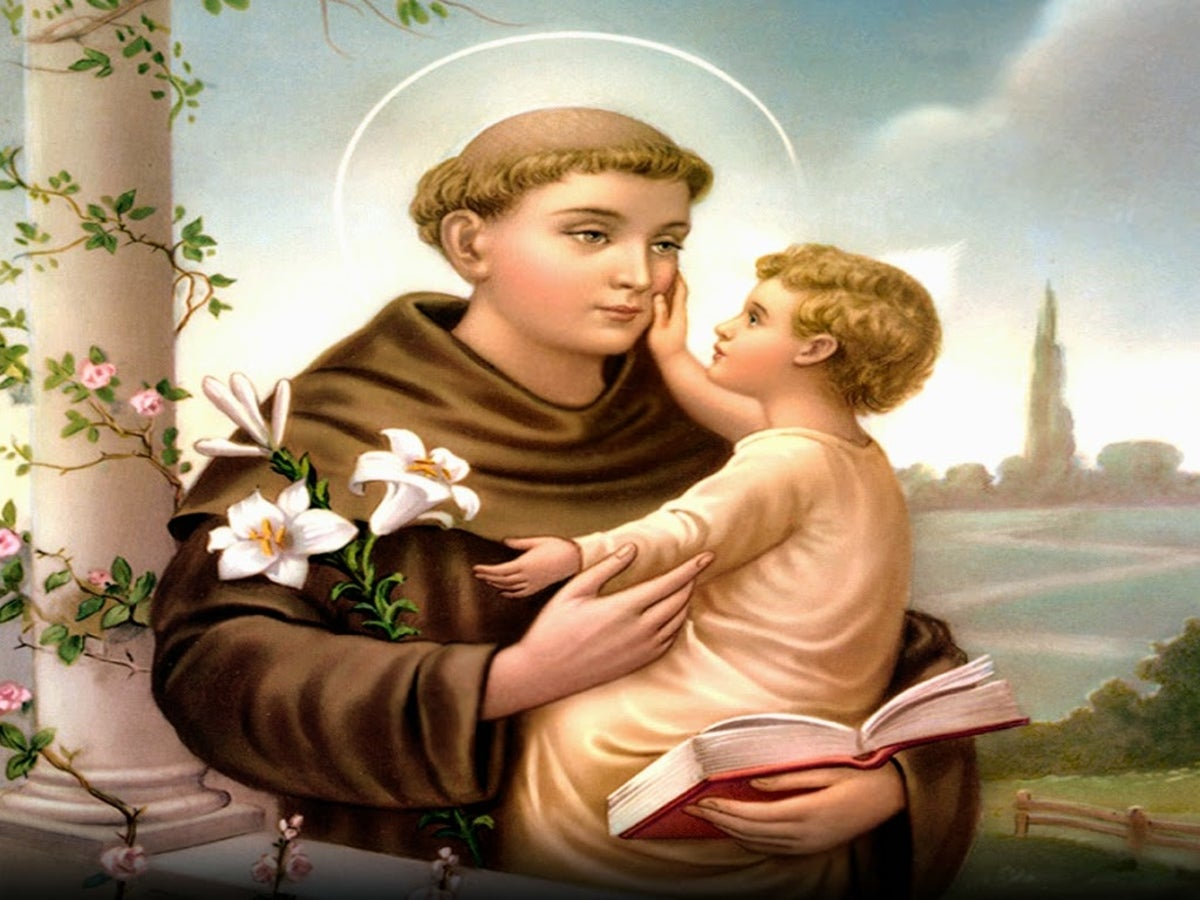
\includegraphics[scale=1, width=.7\textwidth]{san-antonio.jpg}
\end{figure}
\paragraph{}
A todos, Gracias.

% \newpage

\newpage

%%CONTRAPORTADA

{\bfseries \large [Título extendido del TFG (si procede)] }\vspace{10mm} 

{\bfseries \large Resumen:} \vspace{5mm}

Esto es una prueba para probar el formato del Resumen. Esto es una prueba para probar el formato del ResumenEsto es una prueba para probar el formato del ResumenEsto es una prueba para probar el formato del ResumenEsto es una prueba para probar el formato del ResumenEsto es una prueba para probar el formato del ResumenEsto es una prueba para probar el formato del ResumenEsto es una prueba para probar el formato del ResumenEsto es una prueba para probar el formato del ResumenEsto es una prueba para probar el formato del ResumenEsto es una prueba para probar el formato del ResumenEsto es una prueba para probar el formato del ResumenEsto es una prueba para probar el formato del ResumenEsto es una prueba para probar el formato del ResumenEsto es una prueba para probar el formato del Resumen.
\vspace{1cm}

{\bfseries \large Abstract: }\vspace{5mm} 

This is a test to prove the abstract's layout.This is a test to prove the abstract's layout.This is a test to prove the abstract's layout.This is a test to prove the abstract's layout.This is a test to prove the abstract's layout.This is a test to prove the abstract's layout.This is a test to prove the abstract's layout.This is a test to prove the abstract's layout.This is a test to prove the abstract's layout.This is a test to prove the abstract's layout.This is a test to prove the abstract's layout.This is a test to prove the abstract's layout.This is a test to prove the abstract's layout.This is a test to prove the abstract's layout.This is a test to prove the abstract's layout.This is a test to prove the abstract's layout.This is a test to prove the abstract's layout.This is a test to prove the abstract's layout.This is a test to prove the abstract's layout.
\vspace{1cm}

%%Comentar estas notas para que no salgan en la memoria
{\Large\textbf{Nota: el título extendido (si procede), el resumen y el abstract deben estar en una misma página y su extensión no debe superar una página. Tamaño mínimo 11pto.}}
\vspace{1cm}

{\Large\textbf{Extensión máxima 50 páginas sin contar portada, contraportada y declaración responsable (sí se incluye índice, introducción, conclusiones y bibliografía}}
\newpage

%%Incluir aquí la declaración responsable de autoría y uso de las herramientas de IA.
% 
% {\bfseries \large INCLUIR AQUÍ la Declaración Responsable sobre Autoría y Uso Ético de Herramientas de Inteligencia Artificial}
% \vspace{1cm}
% 
% El documento se puede descargar en la página web: https://fisicas.ucm.es/tfg-gradoiec
% \vspace{1cm}
% 
% Y en https://fisicas.ucm.es/file/declaracion-responsable-sobre-autoria-y-uso-etico-de-ia?ver

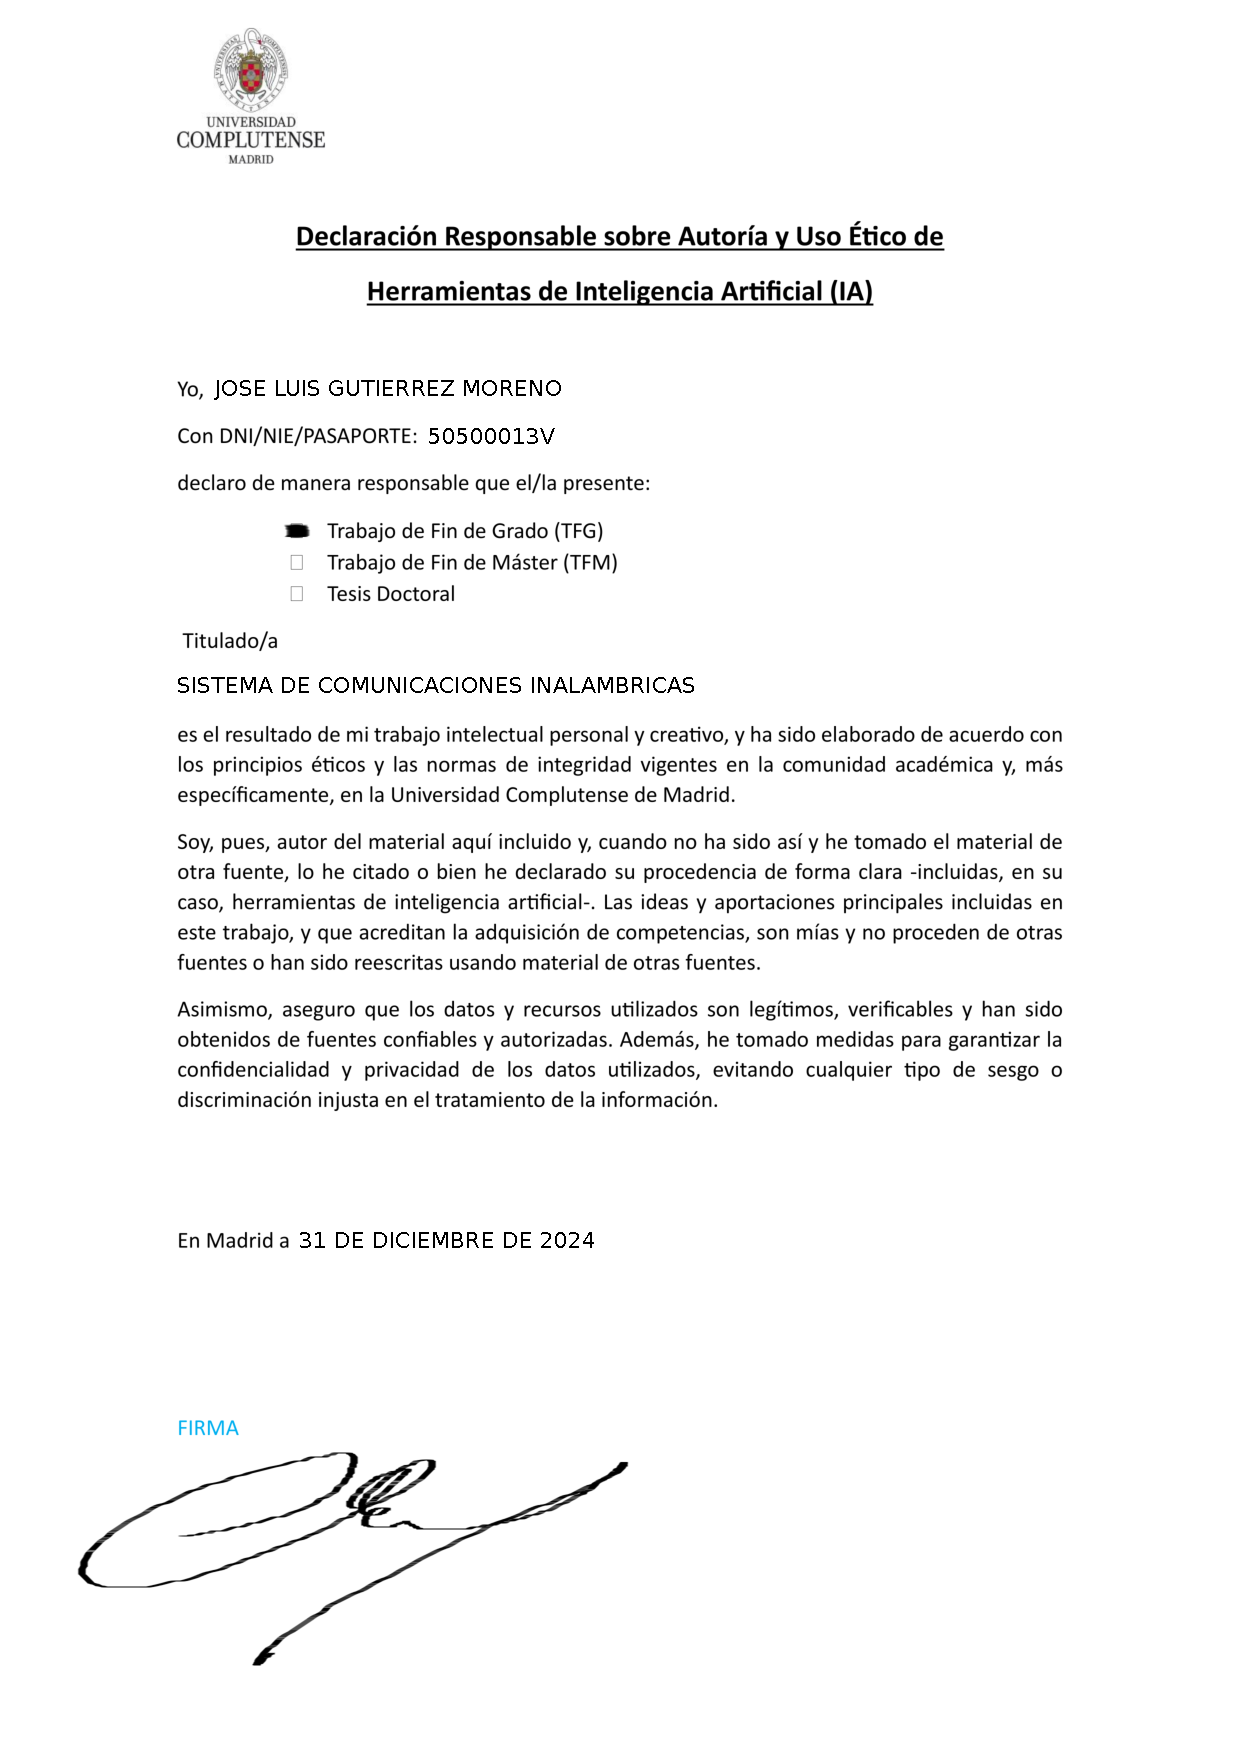
\includegraphics[width=1\textwidth]{./normas-documentacion/iadeclaracion.pdf}
\newpage


\tableofcontents

\newpage


\section{Introducción}
   \label{sec:intro}
   explicacion del problema (calefactor) aplicacion, diagrama de bloques general, explicacion de funciones
Este proyecto se trata de un sistema de comunicaciones de radio digital que pretende ser un circuito de control inalámbrico para aplicaciones generales. 
La base del proyecto es la realización al mayor bajo nivel posible, es decir, desarrollar los dispositivos desde cero.
El sistema de comunicaciones se compone de emisor y receptor. Estos poseen una estructura similar. Una etapa analógica que trabaja con las señales de radio y una etapa digital, basada en un microcontrolador programable. Este microcontrolador implementa la codificación del sistema y trabaja con las señales en banda base.
En la figura REF se muestra un diagrama general de bloques del proyecto.

   \subsection{Objetivos y motivaci\'on}
   objetivos: comprension de los conceptos teoricos, diseno propio basado en los bloques teoricos, solido y funcional 
motivacion: interes por las bases y las comunicaciones inalambricas.
Ensamblaje de todos los conocimientos de las diferentes asignaturas de la carrera.
Aplicación real de la teoría. Acercamiento a la realidad.

\paragraph{}
La elección de este proyecto me llama la atención tanto por mi interés en las bases y las comunicaciones inalámbricas. 
Además por la lilbertad sujeta al proyecto, permite realizar un proyecto creativo y personal, en este caso resolviendo un problema real.
Los objetivos del proyecto son los siguientes:
\begin{enumerate}
\item Recorrer enteramente el proceso de diseño de un sistema de comunicaciones de radiofrecuencia. Al más bajo nivel posible.
\item Resolución de los problemas adjuntos al proceso de diseño.
\item Poner en práctica todos los conceptos teóricos adquiridos posibles.
\item Relacionar los diferentes campos estudiados en el grado.
\item Realización de una aplicaci\'on real y funcional.
\end{enumerate}

\section{Marco Teórico}
   %\paragraph{}
En este apartado se desarrollarán los fundamentos teóricos requeridos para el trabajo.

   \subsection{Sistemas de comunicaci\'on y Transmisión ASK}
   teoria FM, en fsk, demodulacion coherente, ventajas e inconvenientes frente a otras modulaciones, por que de la eleccion de frecuencia 4 MHz y su frecuencia intermedia

caracteristicas selectividad, fiabilidad etc libro 1970 radio amateur pag 94

modulacion ask

\paragraph{}
Una comunicación inalámbrica tiene como objetivo el intercambio de información a través de un medio de propagación no guiado.
En este trabajo, se realizará la comunicación inalámbrica por medio de radiofrecuencia. Esta técnica consiste en acoplar la señal eléctrica que contiene la información a transmitir, a una señal de alta frecuencia. La señal de información se denomina moduladora, mientras que la señal de radiofrecuencia es llamada portadora. La señal eléctrica de información se denomina moduladora y la acción de separar la señal portadora de la moduladora se denomina demodulación.
\paragraph{}
Los elementos que realizan la comunicación son emisor y receptor. La calidad de estos elementos viene definida por las siguientes características:
\paragraph{Receptor:}Las características principales que definen a un buen receptor son: \textbf{Sensibilidad}, propiedad de recibir señales débiles; \textbf{Selectividad:} Propiedad de distinguir entre señales muy próximas en frecuencia, y \textbf{Estabilidad:} Propiedad de mantener de manera fiable una comunicación a lo largo del tiempo.
\paragraph{}
Cabe mencionar que, por la forma de diseño, los receptores se pueden clasificar en función del tipo de detección utilizada: regenerativos y super-regenerativos, que normalmente utilizan una conversión directa, 
o heterodinos y super-heterodinos, los cuales convierten la señal de radiofrecuencia recibida en una señal de frecuencia intermedia, favoreciendo el grado de selectividad principalmente. En general, los receptores super-heterodinos presentan mejores prestaciones a costa de una complejidad y coste mayor.

\paragraph{Transmisor:}La característica principal que define a un buen transmisor es la eficiencia de radiación. Esta medida es la relación entre la potencia transmitida a la antena y la potencia total consumida por el mismo. Idealmente este parámetro es: $\eta = \frac{P_{rad}}{P_{in}} = 1$. La potencia radiada, en esencia, es la potencia que se emite al canal de comunicación. Si se mantiene la eficiencia de radiación, y se aumenta la potencia del transmisor, se consigue un aumento lineal de la potencia radiada. Como resultado, se hace llegar la comunicación a mayor distancia. 
\paragraph{}
También existen otros parámetros que se pueden considerar heredados, ya que son más propios de las antenas, como por ejemplo, la directividad. La mejora de estos parámetros es sustancial a la hora de diseñar un buen receptor.

\paragraph{Modulación ASK}
La modulación ASK es un tipo de modulación digital que se basa en la transmisión de una señal digital en función de la emisión conmutada de una señal portadora, donde la recepción de esta señal representa un símbolo lógico, mientras que su ausencia representa otro.
El esquema de la comunicación ASK se representa en la figura \ref{fig:ask}.

\begin{figure}[h]
    \centering
    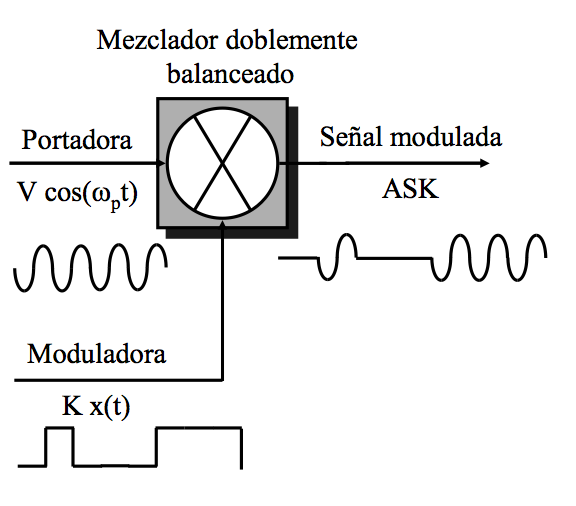
\includegraphics[scale=1, width=.3\textwidth]{ask}
    \caption{Esquema de una posible modulaci\'on ASK}
    \label{fig:ask}
\end{figure}
\paragraph{}

   \subsection{Transistores y sus parámetros característicos}
   \label{sec:teo_transistor}
   \paragraph{}
Un transistor es un dispositivo semiconductor de tres terminales, entrada, salida y terminal común, capaz de amplificar la corriente que circula a través de él. 
Las numerosas técnicas de fabricación de estos dispositivos, dan lugar a los distintos tipos de transistores que existen: BJT, MOSFET, JFET, entre otros.
En este trabajo se utilizarán transistores bipolares BJT, tanto NPN como PNP, para la realización del enlace de radio frecuencia, mientras que, el microconrtolador utilizado en el apartado digital, utiliza principalmente transistores de efecto campo MOSFET.
\paragraph{}
Los transistores BJT logran la amplificación gracias a dos uniones p-n interconectadas entre sí, donde, un pequeño flujo de corriente de entrada, regula un gran flujo de corriente de salida. Por otro lado, en un transistor MOSFET la amplificación se logra por medio de la regulación del estrechamiento del canal por donde circula la corriente, aplicando una tensión inversa.
\paragraph{Polarizaci\'on:}
Para lograr que un transistor realice la función de amplificación, es necesario proporcionar al dispositivo, las tensiones de trabajo adecuadas para que funcione de forma deseada. Esta acci\'on es conocida como polarizaci\'on del transistor.
En función de la polarización aplicada, el transistor puede trabajar de diferentes formas, algunas de las cuales son: activa directa, donde se trabaja en amplificación de señales; o corte y saturación, que son utilizadas principalmente en circuitos digitales.
Existen numerosas técnicas para lograr la polarización deseada, estas serán expuestas en los apartados de desarrollo correspondientes.

\paragraph{Modelo de gran señal del transistor bipolar:}
Existen numerosos modelos matemáticos para definir el comportamiento de un transistor, en este trabajo se utilizará el modelo SPICE del transistor caracterizado por el siguiente modelo circuital y sus ecuaciones características:
\begin{align*} 
   I_E &= \frac { I_{be} }{ B_F } + I_{be} - I_{bc}   & I_{be} &= I_s \cdot \left(e^{\left(\frac {V_{BE}}{N_{T} \cdot V_t} \right)} - 1\right)\\
   I_C &= I_{be} - \frac{I_{bc}}{B_R} - I_{bc}  & I_{bc} &= I_s \cdot \left(e^{\left(\frac {V_{BC}}{N_{T} \cdot V_t} \right)} - 1\right)\\
   I_B &= \frac{I_{be}}{B_F} + \frac{I_{bc}}{B_R} 
\end{align*}

Considerando una polarización en activa directa, donde la amplificación de señales se realiza de manera óptima, las ecuaciones quedan simplificadas al despreciar $I_{bc}$, ya que $V_{CB} < 0$. El resultado de las ecuaciones, a las cuales se aplica el efecto Early, que no se puede considerar despreciable, queda de la siguiente forma. 
\begin{align} 
   \label{eq:1}
   I_C &= I_s \cdot \left(e^{\left(\frac {V_{BE}}{N_{T} \cdot V_t} \right)} - 1\right) \cdot \left(1 + \frac{V_{CE}} {V_{AF}} \right)\\ 
   \label{eq:2}
   I_B &= \frac{I_s}{B_F} \cdot \left(e^{\left(\frac {V_{BE}}{N_{T} \cdot V_t} \right)} - 1\right)
\end{align}

\paragraph{Pequeña señal:}
Como se ha mencionado anteriormente, si se dispone de un transistor que trabaja en activa directa, se consigue la amplificación de las señales. 
Debido a que el transitor es un dispositivo no lineal, la señal introducida debe ser suficientemente pequeña para poder aproximar al dispositivo como un elemento lineal.
Por tanto, a la hora de trabajar con pequeña señal, se modelará al transistor como un cuadripolo lineal de dos puertos. 
En función de las variables de entrada o salida que se elijan, el modelo circuital del cuadripolo variará. El modelo principal con el que se trabajará será el de parámetros híbridos, el cual, se caracteriza por usar como variables independientes $i_1, v_2$ y dependientes $i_2, v_1$. Cabe mencionar la existencia de otras configuraciones de parámetros característicos como son el modelo de admitancias, cuyas variables independientes son $v_1, v_2$, o el modelo de impedancias, cuyas variables independientes son $i_1, i_2$.
El modelo general del cuadripolo lineal así como sus parámetros de entrada y salida se muestran en la figura \ref{fig:1} a continuaci\'on:
\begin{figure}[h]
    \centering
    
\includegraphics[scale=1, width=.3\textwidth]{1}
    \caption{Representación de un transistor como cuadripolo lineal.}
    \label{fig:1}
\end{figure}
\paragraph{}
En general, las ecuaciones que describen el conjunto de los modelos son:
\begin{align} 
   dY_1 = \frac {\partial f_1}{\partial X_1} \cdot \partial X_1 &+ \frac {\partial f_1}{\partial X_2} \cdot \partial X_2 \\ 
   dY_2 = \frac {\partial f_2}{\partial X_1} \cdot \partial X_1 &+ \frac {\partial f_2}{\partial X_2} \cdot \partial X_2 
\end{align}
Donde $X_1$ y $X_2$ corresponden a las variables independientes y $Y_1$ e $Y_2$ a las variables dependientes\\
\paragraph{}
Las ecuaciones que definen al modelo de par\'ametros híbridos en concreto son por tanto:
\begin{align*} 
   v_1 &= h_{11} \cdot i_1 + h_{12} \cdot v_2 \\
   i_2 &= h_{21} \cdot i_1 + h_{22} \cdot v_2
\end{align*}
El valor de los parámetros $h_{nm}$ se deriva de las ecuaciones del modelo de gran señal, simplificadas para una polarización activa directa.
Al derivar dichas ecuaciones se obtiene un modelo de parámetros en admitancias, fácilmente transformable al modelo de parámetros híbridos.
Además, en función de la configuración del terminal común del transistor, el valor de los parámetros característicos cambiará, en este caso, se supondrá una configuración en emisor común. Los valores de los parámetros para las distintas configuraciones pueden ser deducidos utilizando relaciones matemáticas sencillas.
A continuación se expone la obtención de los valores de los parámetros híbridos, para la configuración de emisor común, a partir de las ecuaciones de gran señal, ecuaciones \ref{eq:1} y \ref{eq:2}.
\[
\begin{array}{rcl} 
      \begin{array}{l}
	 \begin{cases}
	    i_b = \frac {\partial I_B}{\partial V_{BE}} \cdot v_{be} + \frac {\partial I_B}{\partial V_{CE}} \cdot v_{ce} \\
	    i_c = \frac {\partial I_C}{\partial V_{BE}} \cdot v_{be} + \frac {\partial I_C}{\partial V_{CE}} \cdot v_{ce} 
	 \end{cases}
      \end{array}
      &
      \begin{array}{l}
	  =>
      \end{array}
      &
      \begin{array}{l}
	 \begin{cases}
	 i_b = y_{11} \cdot v_{be} + y_{12} \cdot v_{ce} \\ 
	 i_c = y_{21} \cdot v_{be} + y_{22} \cdot v_{ce} 
	 \end{cases}
      \end{array}
\end{array}
\]
\[
\begin{array}{rcl} 
      \begin{array}{l}
	 \begin{cases}
	    v_{be} = h_{ie} \cdot i_b + h_{re} \cdot v_{ce} \\
	    i_c = h_{fe} \cdot i_b + h_{oe} \cdot v_{ce}
	 \end{cases}
      \end{array}
      &
      \begin{array}{l}
	  =>
      \end{array}
      &
      \begin{array}{l}
	 \begin{cases}
	    v_{be} = \frac{1}{y_{11}} \cdot i_b + \left(\frac{-y_{12}}{y_{11}}\right) \cdot v_{ce} \\
	    i_c = \frac{y_{21}}{y_{11}} \cdot i_b + \left( y_{22} - \frac{y_{12} \cdot y{21}}{y_{11}}\right) \cdot v_{ce} 
	 \end{cases}
      \end{array}
\end{array}
\]

\paragraph{}
Teniendo en cuenta las relaciones obtenidas, se puede establecer la relación de los parámetros híbridos con su valor numérico como se muestra a continuación.
\begin{align} 
   h_{ie} &= \frac { 1 }{ y_{11} } = \frac{N_F \cdot V_t}{I_B} & h_{re} &= \frac{-y_{12}}{y_{11}} \approx 0 \label{eq:h_param1} \\
   h_{fe} &= \frac { y_{21} }{ y_{11} } = \frac{I_C}{I_B} & h_{oe} &=  y_{22} - \frac{y_{12} \cdot y_{21}}{y_{11}}\approx \frac{I_C}{V_{AF}} \label{eq:h_param2}
\end{align}

\paragraph{}
Seguidamente, se establecen las relaciones de los parámetros híbridos en emisor com\'un para las demás configuraciones de terminal común. Las relaciones se obtienen de manera similar a las anteriores dadas:
   \begin{equation} \label{eq:h_conversion}
%\[
\begin{array}{rrcll} 
      \begin{array}{l}
	 h_{ic} = h_{ie} \\
	 h_{fc} = - (1+ h_{fe} )
      \end{array}
      &
      \begin{array}{l}
	 h_{rc} = 1 - h_{re} \\
	 h_{oc} = h_{oe}
      \end{array}
      &
      \begin{array}{l}
	 \bigg|
      \end{array}
      &
      \begin{array}{l}
	 h_{ib} = \frac{h_{ie}}{1+h_{fe}} \\
	 h_{fb} = -\frac{h_{fe}}{1+h_{fe}} 
      \end{array}
      &
      \begin{array}{l}
	 h_{rb} = \frac{h_{ie} \cdot h_{oe}}{1+h_{fe}} - h_{re}\\
	 h_{ob} = \frac{h_{oe}}{1+h_{fe}} 
      \end{array}
\end{array}
%\]
   \end{equation}

Por último, cabe mencionar que los transistores por su construcción física poseen elementos denominados parásitos. Estos elementos se modelan, de manera circuital principalmente como condensadores, y pueden influir en los valores de las impedancias de entrada, salida o realimentaciones. Estos efectos se incluirán cuando sean necesarios en el desarrollo del proyecto.

   \subsection{Realimentaci\'on}
   \label{sec:teo_osc}
   libro Paul R. Gray, Paul J. Hurst, Stephen H. Lewis, Robert G. Meyer - Analysis and Design of Analog Integrated Circuits (2001, Wiley) capitulo feedback revista todoelectronica fasciculo segundo.
\paragraph{}
La realimentación es un concepto ligado a la amplificación.
La realimentación, en los amplificadores, consiste en tomar una muestra de tensión o de corriente a la salida y reenviarla a la entrada a través de una red apropiada.
gracias a la realimentación se consigue estabilizar la ganancia, la resistencia de entrada, la resistencia de salida y el ancho de banda, aunque el fin más importante es la estabilización de la ganancia.
\paragraph{}
En la figura \ref{fig:fb} se muestra el esquema general de un sistema realimentado. Donde $A$ se corresponde con la ganancia en lazo abierto del amplificador, y $f$ la red de realimentaci\'on correspondiente. Dependiendo de la naturaleza del amplificador y del tipo de realimentación, la ganancia en lazo abierto puede ser de tensión, corriente, transimpedancia o transconductancia.
\begin{figure}[h]
    \centering
    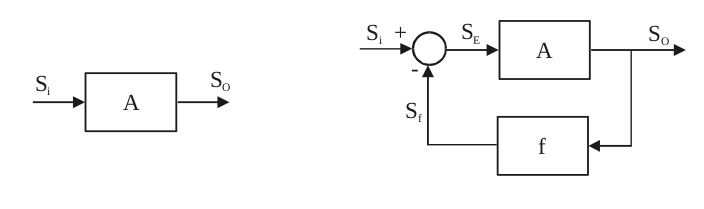
\includegraphics[scale=1, width=.7\textwidth]{fb}
    \caption{a) Amplificador sin realimentaci\'on, b) Sistema realimentado} 
    \label{fig:fb}
\end{figure}
\paragraph{}
Se calculan las ganancias propias de cada sistema en la figura \ref{fig:fb}. La nomenclatura $S_n$ se refiere a una señal que bien puede ser de corriente o tensión.
Por un lado, la ganancia en lazo abierto del amplificador se calcula como:
$$A = \frac{S_o}{S_i} $$
Por otro lado, se calcula la ganancia en lazo cerrado $A_f$:
\[
\begin{array}{rccl} 
      \begin{array}{l}
	 \begin{cases}
	    S_f = S_o \cdot f \\
	    S_E = S_i - S_f \\
	    S_o = S_E \cdot A
	 \end{cases}
      \end{array}
      &
      \begin{array}{l}
	  =>
      \end{array}
      &
      \begin{array}{l}
	 \frac{S_o}{A} = S_i - S_o \cdot f \\
	 S_i = S_o \cdot \left(\frac{1}{A} + f \right) = S_o \cdot \frac{1}{A} \cdot (1 + f \cdot A) \\
	 A_f = \frac{S_o}{S_i}
      \end{array}
      &
      \begin{array}{l}
	 A_f = \frac{S_o}{S_i} = \frac{A}{(1 + f \cdot A)} 
      \end{array}
\end{array}
\]
\paragraph{}
Se señalan las ecuaciones que ser\'an de utilidad:
\begin{align}
   \label{eq:feedback}
   A_f &= \frac{S_o}{S_i} = \frac{A}{(1 + f \cdot A)} \\
   \label{eq:A}
   A &= \frac{S_o}{S_E} \\
   \label{eq:Al}
   A_l &= A \cdot f
\end{align}
\paragraph{}
Es útil definir el par\'ametro ganancia en lazo abierto, $A_l = A \cdot f$, para poder analizar el comportamiento del sistema en lazo cerrado cuando $A_l$ var\'ia. Esto se conoce como el criterio de Barkhausen, el cual se expone considerando el criterio de signos de la ecuaci\'on \ref{eq:feedback}:
\begin{itemize}
   \item \textbf{Si $\mathbf {A_l >> 1}$:} en este caso se obtiene una ganancia total del sistema $A_f = \frac{1}{f}$. Esta realimentación se conoce como negativa.
   \item \textbf{Si $\mathbf{A_l << 0}$:} en este caso se tiene que $S_E = S_i + S_f$, es decir, las señales se encuentran en fase y se suman en lugar de restarse. Esta suma es amplificada una y otra vez dando lugar a un sistema inestable. Esta realimentación se conoce como positiva.
   \item \textbf{Si $\mathbf{A_l = -1}$:} en este caso se el sistema se encuentra en la frontera entre la estabilidad y la inestabilidad. Por lo que idealmente, el sistema responder\'a a la funci\'on impulso o delta de Dirac con una oscilaci\'on continuada. Este caso es conocido como el criterio de Barkhausen y se trata de la condici\'on necesaria para encontrar oscilaciones.
\end{itemize}
\paragraph{}
Por último se han de mencionar los diferentes tipos de realimentación que se dan en los amplificadores prácticos. Como se ha mencionado anteriormente, las señales de trabajo pueden ser de tensión, corriente o incluso una combinación de ambas. De esta forma, se pueden clasificar los diferentes tipos de realimentación en función de la señal de trabajo tanto a la entrada como a la salida. Alugnos de estos tipos se exponen en las figuras \ref{fig:sp} y \ref{fig:pp}.
\begin{figure}[H]
    \centering
    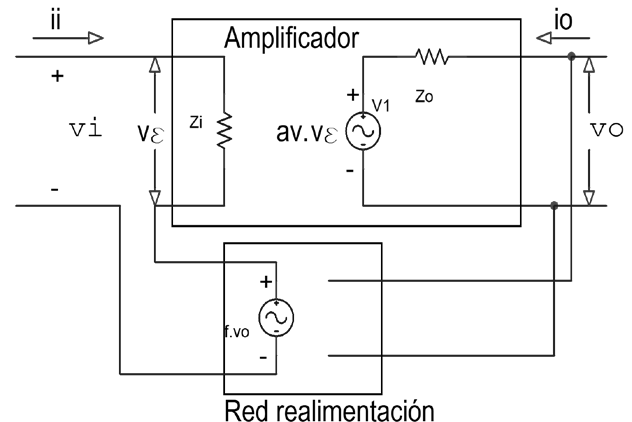
\includegraphics[scale=1, width=.4\textwidth]{sp-tension}
    \caption{Amplificador de tensión con realimentaci\'on serie paralelo ideal.} 
    \label{fig:sp}
\end{figure}

\begin{figure}[H]
    \centering
    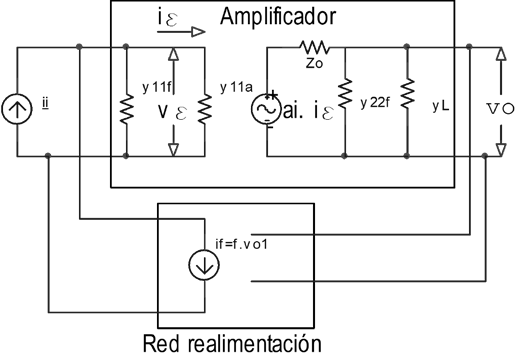
\includegraphics[scale=1, width=.4\textwidth]{pp-transres-real}
    \caption{Amplificador de transresistencia con realimentación paralelo paralelo real.} 
    \label{fig:pp}
\end{figure}

   \subsection{Sistemas integrados: Atmega328p}
   %Digital Design and Computer Architecture capitulo 4; datasheet atmega
\paragraph{}
Un sistema integrado o embebido es un sistema digital complejo, compuesto principalmente por CPU, memoria, buses y perif\'ericos, entre otros. La conjunción específica del sistema se denomina arquitectura. El conjunto de los elementos del sistema tambi\'en es conocido como SOC (\textit{System On Chip}).
\begin{figure}[h]
    \centering
    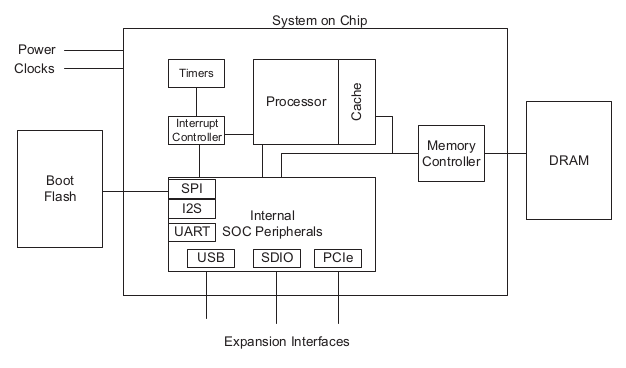
\includegraphics[scale=1, width=.6\textwidth]{soc}
    \caption{Esquema general de un SOC.} 
    \label{fig:soc}
\end{figure}
\paragraph{}
A continuaci\'on se realiza una descripción de los elementos principales que componen el SOC:
\begin{itemize}
\item \textbf{CPU:} Un sistema integrado posee al menos una CPU, la cual se encarga de la ejecuci\'on de los programas, operando con datos e instrucciones. Dependiendo del diseño de la CPU, se tiene una arquitectura de $n$ bits, lo cual implica que el tamaño de los registros y de las direcciones es de $n$ bits. El diseño de la CPU también especifica el uso de un repertorio de instrucciones concreto. Algunos ejemplos de repertorio de instrucciones son ARM, MIPS o CISC. La CPU se consolida como el principal elemento de la arquitectura.
\paragraph{}
   A pesar de que la CPU constituya el elemento principal del sistema integrado, para que todo su procesamiento de datos resulte en trabajo \'util, es necesario el soporte de hardware externo. Dentro de este conjunto de hardware se pueden distinguir:
\item \textbf{Subsistema de memoria:} La memoria en general se encarga de almacenar y servir los datos e instrucciones utilizadas por el procesador. El sistema de memoria se puede descomponer en varios m\'odulos, como por ejemplo: la memoria cach\'e, una memoria f\'isicamente al lado del procesador con una velocidad de trabajo de unos pocos ciclos de procesador; la memoria DRAM, un dispositivo de memoria con un espacio de almacenamiento mayor que la cach\'e, aunque normalmente un orden de magnitud m\'as lenta, u otras memorias externas de diferentes tipos como pueden ser SRAM, FLASH o ROM.
\item \textbf{Controlador de interrupciones:} Este mecanismo gestiona los requerimientos de atención del procesador por parte de los dispositivos, sin necesidad de que este tenga que estar pendiente de la falta de atención continuamente.
\item \textbf{Timers:} El objetivo de estos dispositivos es generar una frecuencia de onda cuadrada estable. Estos dispositivos son imprescindibles para el funcionamiento de la CPU, ya que controlan la frecuencia de trabajo del procesador, o incluso otras tareas como las interrupciones periódicas, programación de eventos o la fecha y hora.
\end{itemize}
\paragraph{Mapa de memoria:} El mapa de memoria es la lista de direcciones accesibles de todos los elementos del sistema: DRAM, controlador de interrupciones... El tamaño total del mapa de memoria dependerá del tipo de arquitectura del procesador y se calcula como $2^n$. Cuando el procesador ejecuta una instrucción de lectura o escritura, la dirección es decodificada por los decodificadores y finalmente enrutada hacia el correspondiente elemento del sistema\footnote{Harris, D. M., & Harris, S. L. (2012). \textit{Digital Design and Computer Architecture} Capítulo 4.}.

\paragraph{AVR Atmega328p:} Como ejemplo de un sistema integrado, se introduce el procesador Atmega328p, el cual he utilizado en el proyecto. 
En las figura \ref{fig:avr-cpu} se muestra un esquema general del sistema integrado Atmega328p. 
\begin{figure}[h]
    \centering
    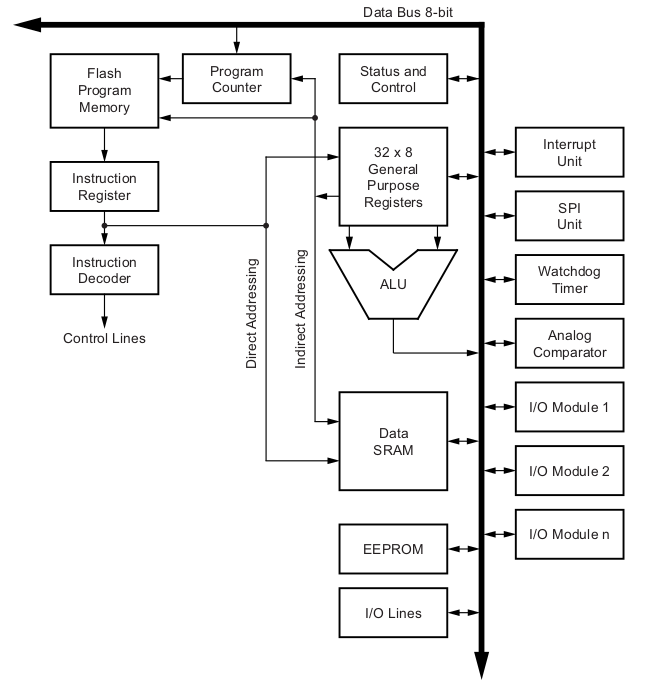
\includegraphics[scale=1, width=.7\textwidth]{avr-cpu}
    \caption{Diagrama de bloques del Atmega328p, en detalle la CPU}
    \label{fig:avr-cpu}
\end{figure}
El Atmega328p es un sistema integrado tipo RISC con un procesador de 8 bit, el cual es capaz de ejecutar una instrucci\'on por ciclo. Esto es posible gracias al diseño de una arquitectura tipo harvard, la cual se caracteriza por disponer de memorias separadas para datos y para las instrucciones del programa. Las instrucciones son ejecutadas con un nivel de segmentaci\'on, lo que permite que, mientras una instrucción está siendo ejecutada, la siguiente instrucción está siendo buscada en la memoria de programa. Es necesario aclarar que la CPU es capaz de trabajar con registros dobles, siendo capaz de direccionar un total de $2^{16}$ posiciones de memoria.
\paragraph{}
Como se puede apreciar en la figura \ref{fig:avr-cpu}, el bloque \textit{Flash program memory} (memoria flash) se corresponde con el espacio de almacenamiento donde se encuentran las instrucciones de nuestro software. Seguidamente se encuentra \textit{Instruction register}, que permite el nivel de segmentaci\'on de las instrucciones. Continuando el esquema, La instrucci\'on a ejecutar es decodificada siguiendo el mapa de memoria y correctamente enrutada al dispositivo correspondiente mediante \textit{Instruction decoder}.
\paragraph{}
Una vez la instrucci\'on es decodificada, pasa a ser ejecutada, entrando en escena la parte de datos. El bloque de los registros, \textit{General purpose Registers} sirven de operandos y junto al bloque \textit{ALU}, se encargan de realizar las operaciones que se requieran. Una vez generados los datos, se vuelcan en el bus de datos y ser\'an recogidos por el dispositivo interesado, gobernados por \textit{Control Lines}. La lectura de los operandos, la operaci\'on con la \textit{ALU} y la escritura del resultado en el banco de registros, se realiza en un solo ciclo de reloj. El \textit{Status Register} es un registro que se actualiza en cada operaci\'on aritm\'etica con las particularidades de dicha operaci\'on: bit $zero$, $carry$, $overflow$, incluso la habilitaci\'on de las interrupciones globales.
\paragraph{}
Como se ha comentado, existen dos mapas de memoria bien diferenciados: instrucciones y datos. La memoria de instrucciones es la flash, la cual tiene una capacidad de $2^{15} \unit{\byte} \approx \SI{32}{\kilo\byte}$, por lo que todas las direcciones de memoria est\'an dedicadas a este elemento.
Por otro lado, se tiene el mapa de memoria de datos, estructurado de la forma mostrada en la figura \ref{fig:mem_datos}.
\begin{figure}[h]
    \centering
    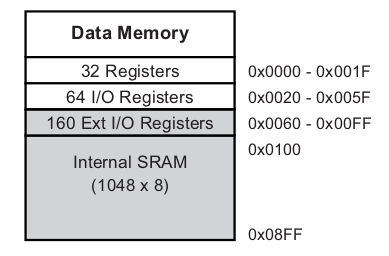
\includegraphics[scale=1, width=.3\textwidth]{avr_datos}
    \caption{Mapa de memoria de datos direccionada por bytes}
    \label{fig:mem_datos}
\end{figure}
Se puede observar en la figura \ref{fig:mem_datos} que el mapa de memoria de datos est\'a separado en distintas regiones: para el banco de registros, para los dispositivos de entrada salida y para la \textit{SRAM}. La \textit{SRAM} es la memoria f\'isica de datos y posee una capacidad de \SI{2}{\kilo\byte}. Al igual que la \textit{FLASH}, esta memoria es accedida mediante registros dobles. El soporte para lidiar con datos de 16 bits se realiza por medio de unos registros especiales, nombrados como X, Y y Z\footnote{Atmel. (n.d.). \textit{ATmega328P Automotive Microcontrollers Datasheet} (Atmel-7810). Recuperado de \url{https://www.microchip.com/wwwproducts/en/ATmega328P}.}.

\newpage
\section{Desarrollo}
   \paragraph{}
En este apartado se desarrollar\'an los diferentes módulos que componen el sistema.
Como se ha introducido en el apartado \ref{sec:intro}, el sistema de comunicaciones consta de un emisor y receptor que comparten la misma estructura de diseño: 
una parte analógica que actúa como la interfaz de comunicación de radiofrecuencia y una parte digital que trabaja con las señales banda base. Además, la parte digital también se encarga de la codificación y decodificación del enlace.
En cuanto a la parte analógica de radiofrecuencia nos encontramos las siguientes características generales que se desarrollan en los consiguientes apartados. 
La comunicaci\'on que se llevará a cabo consiste en un enlace digital mediante radio frecuencia de dos canales.
La frecuencia de trabajo es de \SI{30}{\mega\hertz} sobre una modulación es ASK.
Esta modulación implica que el sistema analógico de radio trabaja recibiendo tonos sintonizados a la frecuencia de trabajo.
Por otro lado, la parte digital, trabaja tanto con
la codificación en la parte emisora, como con demodulación de las señales digitales en la parte receptora. 
La codificación y demodulación se realiza con ayuda de un microcontrolador Atmega328p, el cual, mediante las señales producidas por dos distintos pulsadores, codifica la señal digital de manera NRZ apolar.
Esta señal es posteriormente demodulada y decodificada en el receptor.
Se muestra, en la figura \ref{fig:bloques_gral}, un diagrama de bloques como esquema general de ambas partes del proyecto, transmisor y receptor. En ambos casos se diferencian la parte digital y anal\'ogica en cada caso.

\begin{figure}[h]
    \centering
    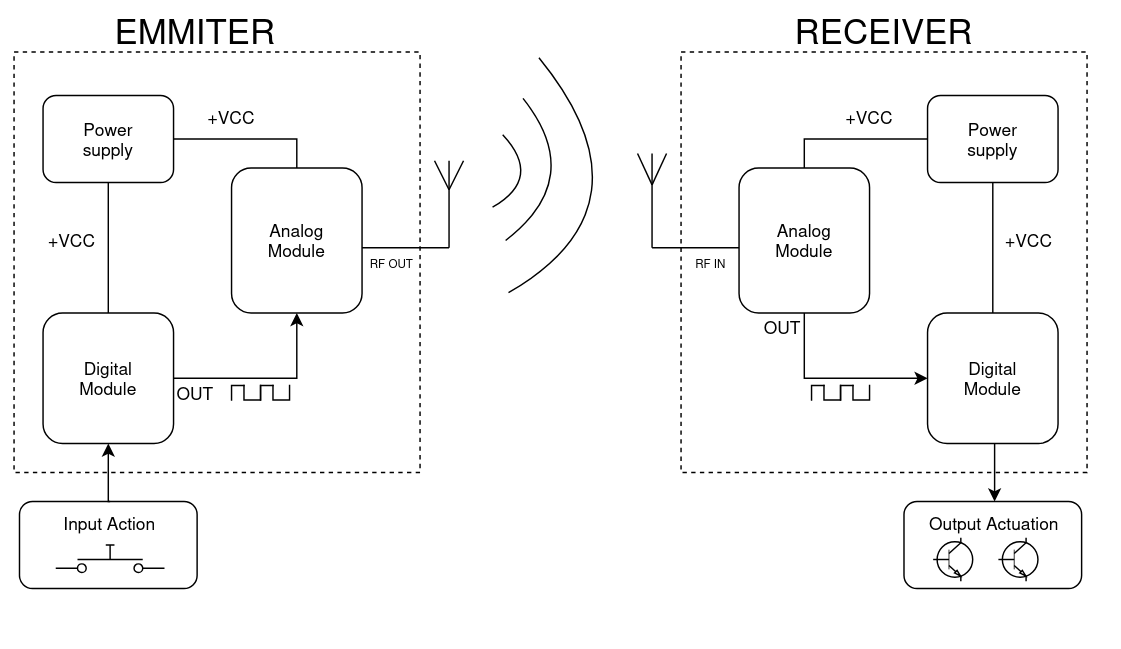
\includegraphics[scale=1, width=1\textwidth]{bloques_gral}
    \caption{Diagrama de bloques general del proyecto}
    \label{fig:bloques_gral}
\end{figure}

   \subsection{Parte anal\'ogica}
   \paragraph{} En este apartado se desarrolla todo lo referente a la interfaz de radiofrecuencia (RF). En primer lugar, se explica de manera analítica el funcionamiento del transmisor y receptor, para posteriormente realizar un análisis cuantitativo, llevando a cabo los cálculos correspondientes a los valores de los componentes del sistema.

\paragraph{Transmisor:} El transmisor está basado en un oscilador de un solo transistor en base com\'un sintonizado por un circuito $LC$, conocido como circuito tanque.
Los valores del condensador e inductancia del circuito tanque poseen una frecuencia de resonancia, la cual se amplificar\'a por medio de la realimentación positiva. La oscilación es cortada eléctricamente a conveniencia por medio de otro transistor, produciendo una modulación AM-ASK. El transmisor se diseña de forma que radie la mayor potencia posible, y en consecuencia, propagar la señal a la mayor distancia posible.

\paragraph{Receptor super-regenerativo:} El receptor super-regenerativo, diseñado en 1920, se basa en el concepto de realimentación positiva. Sin embargo, su antecesor, el receptor regenerativo, consiste en diseñar un bucle de realimentación cuyo Al sea $A_l = 1$ (explicaci\'on en el apartado \ref{sec:teo_osc}), dotando a este receptor de gran sensibilidad a la frecuencia de resonancia. 
El receptor regenerativo, en la práctica, es muy complicado de llevar a su condici\'on de trabajo, $A_l = 1$, pues las mínimas variaciones harán que el circuito comience a oscilar o no ser tan sensible. Por este hecho se desarrolla el receptor super-regenerativo, que se basa en este mismo concepto de realimentación positiva, con la diferencia de que, en este caso, $A_l > 1$ permitiendo en consecuencia, la oscilaci\'on. Pasado un determinado tiempo, el circuito corta la oscilación, permitiendo que el ciclo comience de nuevo. Esta señal de reinicio y paro se denomina \textit{quench-signal}. En cada inicio del periodo de la señal \textit{quench-signal}, momento en el cual la oscilación se está generando, el circuito atraviesa un periodo de sensibilidad máxima a las señales con frecuencia igual a la de resonancia. Si una señal es detectada, la oscilación del circuito se producirá de forma más rápida, aumentando así la frecuencia de la \textit{quench-signal}, obteniendo como salida una señal con modulación FM con frecuencia de la \textit{quench-signal}.

%\paragraph{} Eleccion de frecuencia 33MHz (sistemas de radio control) El receptor super-regenerativo trabaja mejor con frecuencias mayores pues permite una frecuencia de quench mayor, aumentando la tasa de muestreo. empiricamente cuanto mayor frecuencia mejor diseño de antena optimo mas corto, mejor distancia 

   \subsubsection{Diseño de la parte anal\'ogica de RF del transmisor}
   \label{sec:des_tx}
   datasheets ne555, 2n2222, octave
\paragraph{}
En este apartado se expondr\'a el diseño del transmisor, los c\'alculos matem\'aticos necesarios, simulacion por ordenador y los resultados practicos.
El transmisor está diseñado para generar una modulación ASK y emitir a una frecuencia de $30Mhz$. La frecuencia de emisión se sintoniza con la del receptor por medio de un condensador de capacidad variable.
\paragraph{}
NO REPETIR, EXPLICAR LA FOTO
En la figura \ref{fig:tx} se puede observar el esquema eléctrico del transmisor.
El principio de funcionamiento del transmisor es un oscilador, basado en un par resonante LC, el cual fija la frecuencia de emisión. Esto se realiza realizando un bucle de realimentación positiva, donde el transistor NPN juega el papel de elemento activo de amplificación, el circuito tanque LC es el filtro que permite que en cada iteración del bucle, se amplifique la frecuencia deseada. mientras que el condensador de realimentación, genera la realimentación positiva, sumando una fracción de la salida con la señal de entrada, que en este caso es el propio ruido generado por el circuito.
El circuito se diseña para disipar la mayor potencia posible para que la señal alcance la mayor distancia posible. 
Por otra parte, el cicuito permite modular la señal portadora eléctricamente cortando y produciendo la oscilación en función de las variaciones de la señal moduladora. Esto es posible gracias al segundo transistor PNP, el cual trabaja en corte y saturaci\'on y corta el paso de corriente general del circuito.
% Esto se realiza por medio de un oscilador Colpitts en base común sintonizado a la frecuencia de emisión y que a su vez es mezclado con una señal de onda cuadrada generada por el chip integrado NE555.
% La señal de onda cuadrada generada por el NE555, es modulada en frecuencia, por dos pulsadores, produciendo dos diferentes canales digitales de salida.
El esquema completo del transmisor se expone en la figura \ref{fig:tx}.

\begin{figure}[h]
    \centering
    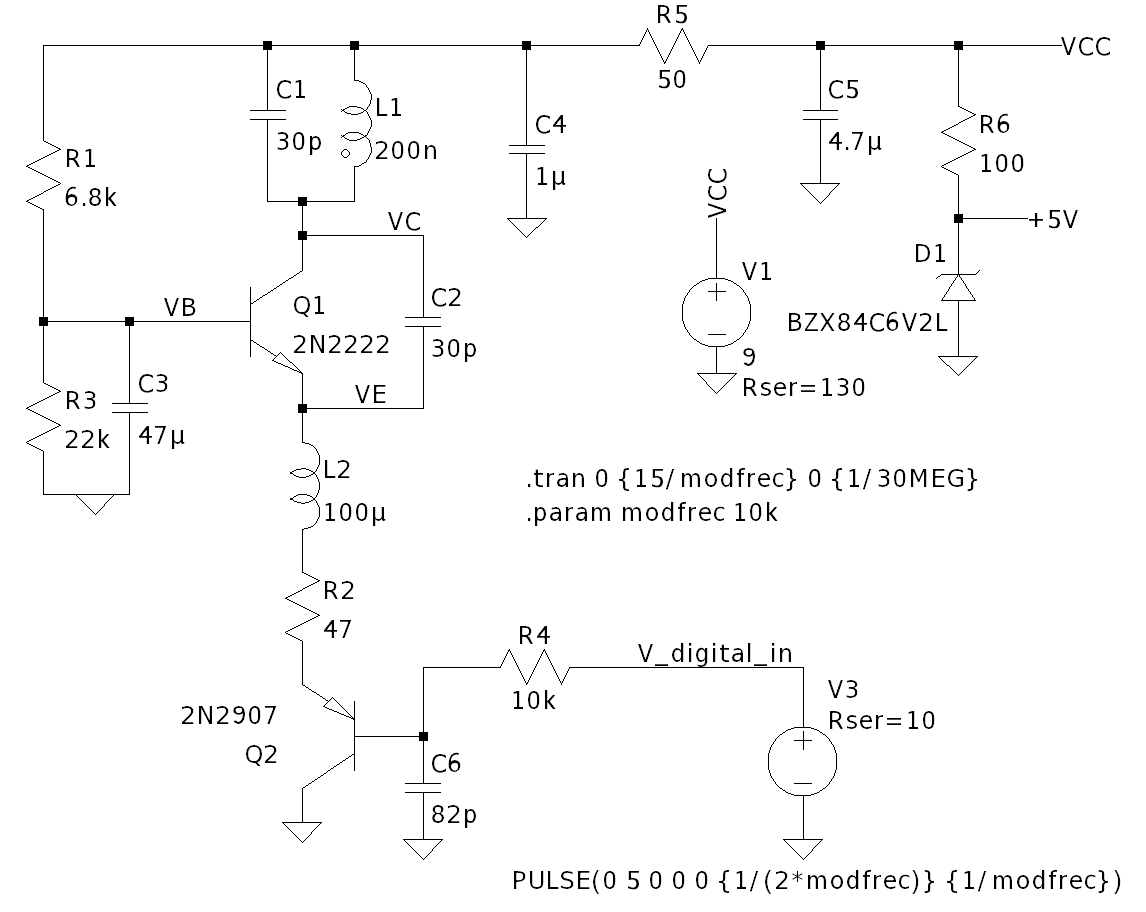
\includegraphics[scale=1, width=1\textwidth]{transmisor}
    \caption{Esquema el\'ectrico del transmisor}
    \label{fig:tx}
\end{figure}

\paragraph{Diseño del oscilador}
\paragraph{Polarizaci\'on:} IGUAL Y MENCIONANDO EL TRANSISTOR PNP EN CORTE APROX 0.2 V DESPRECIABLE.
En primer lugar se debe fijar el punto de operación deseado. Se deben tener encuenta dos cosas: la zona trabajo del transistor y la potencia del circuito. La zona de trabajo debe ser activa directa, pues para producir la oscilación, el bucle de realimentación positiva debe tener la etapa de amplificación proporcionada por el transistor. La potencia del circuito, junto a la fracuencia de diseño, acotan el modelo de transistor que se ajuste al circuito.
En primer lugar se necesita un transistor con una frecuencia de transición $f_t > \SI{30}{\mega\hertz}$. Aparte el parámetro $I_{Cmax}$ debe ser suficiente para proporcionar la potencia deseada sin deteriorarse. Se elige un transistor 2N2222, cuya $f_t > \SI{30}{\mega\hertz}$ e $I_{Cmax} = \SI{0.6}{\ampere}$ y una $V_{CC} = \SI{9}{\volt}$. Se fija $Ic = \SI{80}{\milli\ampere}$, que supondr\'a una potencia de aproximadamente $I_C \cdot V_{CC} = \SI{0.72}{\watt}$ y $V_{CE} = \frac{V_{CC}}{2} = \SI{4.5}{\volt}$ condici\'on necesaria para trabajar en activa directa. Además, de la hoja de características del 2N2222 se conoce $h_{FEmax} \approx 300$, aunque medido con un mult\'imetro, nos da el valor $h_{FE} = 280$ por lo que se utilizar\'a este \'ultimo.
En lugar de repetir el cálculo que se hizo para seleccionar el valor de las resistencias de polarización, se optará por comprobar si los valores elegidos satisfacen las imposiciones.
\paragraph{}
Se utiliza equivalente de Thevenin para las resistencias en paralelo. En la malla que aparece se obtiene:
$$V_{th} - 0.7 - I_c \cdot R_e = I_b \cdot R_{th}$$
Siendo:
\[
\begin{array}{rl} 
      \begin{array}{l}
	 V_{th} = \frac{V_{CC} \cdot R_2}{R_1+R_2} \\
	 R_{th} = \frac{R_1 \cdot R_2}{R_1+R_2}
      \end{array}
      &
      \begin{array}{l}
	 I_b \cdot h_{FE}= I_c \\
	 h_{FE} = 280
      \end{array}
\end{array}
\]
Se obtienen $I_c$ y $V_{CE}$ con las siguientes dos ecuaciones sustituyendo los valores correspondientes:
\begin{align*}
   R_1=\SI{10}{\kilo\ohm} \quad R_2=\SI{20}{\kilo\ohm} \quad &R_E=\SI{40}{\ohm} \quad V_{CC} = \SI{9}{\volt} \\
   I_c \cdot \left( 40+ \frac{R_{th}}{h_{FE}}\right) &= V_{th} - 0.7 \\
   V_{CC} = V_{CE} &+ I_C \cdot R_E \\
   V_{CE}= \SI{5.68}{\volt} \quad& I_C = \SI{83}{\milli\ampere}
\end{align*}
\paragraph{}
Una vez calculado el puto de operaci\'on se obtienen los par\'ametros h\'ibridos en base com\'un siguiendo las ecuaciones expuestas en el apartado \ref{sec:teo_transistor}. Adem\'as se debe calcular el dato $V_{AF}$ con ayuda de la hoja de datos del transistor, en este caso el dato se obtuvo como una media del rango de valores proporcionado. El resultado del c\'alculo de los par\'ametros es el siguiente:
\begin{equation}
   \label{eq:result_pol1}
V_{AF} = \frac{I_{Cdata}}{h_{OEdata}} =\frac{\SI{1}{\milli\ampere}}{\SI{6}{\micro\siemens}} =  \SI{50}{\volt} 
\end{equation}
\begin{equation}
   \label{eq:result_pol2}
%\[
\begin{array}{rl} 
      \begin{array}{l}
	 h_{ib} =  \SI{8.4}{\ohm} \\
	 h_{fb} =  -0.99
      \end{array}
      &
      \begin{array}{l}
	 h_{rb} =  0.014 \\
	 h_{ob} =  \SI{6}{\micro\siemens}
      \end{array}
\end{array}
%\]
\end{equation}

\begin{figure}[h]
    \centering
    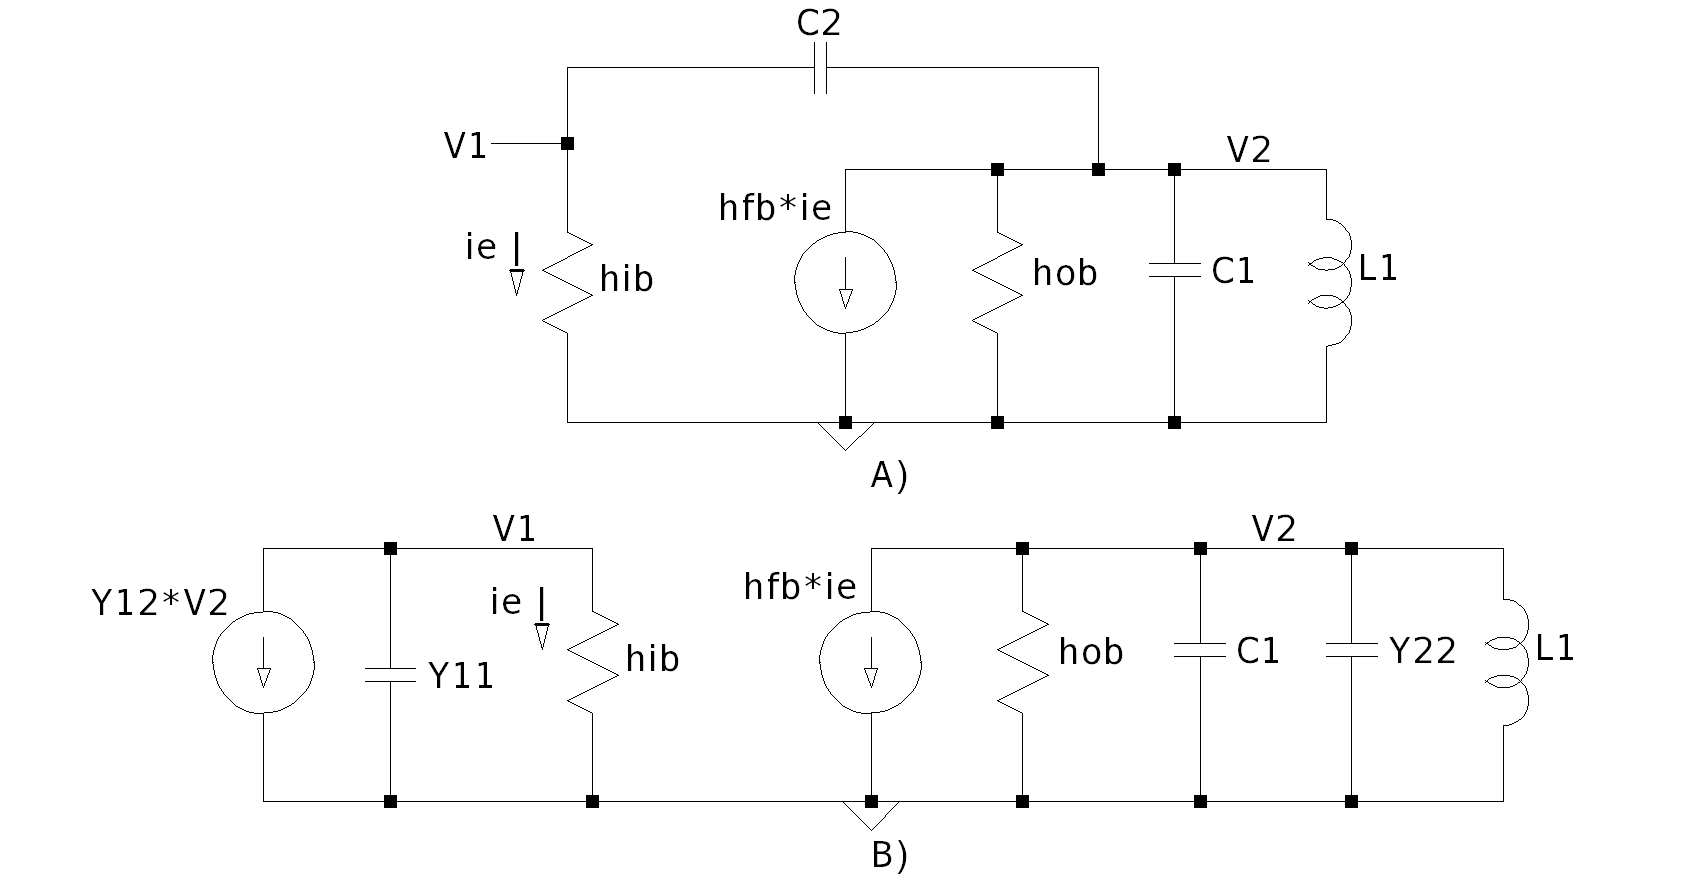
\includegraphics[scale=1, width=.8\textwidth]{small_signal_tx}
    \caption{A) Modelo en pequeña señal del bucle de oscilación para frecuencias medias B) Modelo en pequeña señal del oscilador sustituyendo el condensador de realimentación $C_1$ por su equivalente en parámetros $Y$}
    \label{fig:ss_tx}
\end{figure}

\paragraph{Modelo en pequeña señal:} ANADIR LOS CALCULOS DE LA INDUCTANCIA APROX 200N SEGUN INTERESE. El objetivo de este modelo es el cálculo de la frecuencia de resonancia del oscilador. En la figura \ref{fig:ss_tx} se muestra el modelo en pequeña señal del oscilador para frecuencias intermedias, entorno a la frecuencia de oscilaci\'on. El bucle de oscilaci\'on se trata de una realimentación paralelo-paralelo, por lo que se representa el condensador de realimentación $C_1$ como su equivalente en par\'ametros $Y$. El valor de dichos par\'ametros son:
\[
\begin{array}{rl} 
      \begin{array}{l}
	 Y_{11} = \frac{i_1}{v_1}|_{v_2 = 0} = s \cdot C_2 \\
	 Y_{12} = \frac{i_1}{v_2}|_{v_1 = 0} = -s \cdot C_2 
      \end{array}
      &
      \begin{array}{l}
	 Y_{21} = \frac{i_2}{v_1}|_{v_2 = 0} = -s \cdot C_2 \\
	 Y_{22} = \frac{i_2}{v_2}|_{v_1 = 0} = s \cdot C_2 
      \end{array}
\end{array}
\]
\paragraph{}
Se deben tener en cuenta ciertas consideraciones previas como consecuencia del an\'alisis del esquema B) en la figura \ref{fig:ss_tx}. La realimentaci\'on es positiva en el momento que $Y_{12}<0$ y $h_{fb}<0$ por lo que $V_2>0$. El modelo que se muestra corresponde a frecuencias intermedias entorno a la de oscilaci\'on. Para frecuencias bajas, la impedancia de $C_2$ tendrá un valor tan alto que corta la realimentación ,siguiendo el esquema A) figura \ref{fig:ss_tx}. para frecuencias altas, la impedancia de $C_2$ tendr\'a un valor tan bajo que supondr\'a un cortocircuito a tierra para la corriente de realimentaci\'on, por lo que $ie = 0 \unit{\ampere}$.
\paragraph{}
Se calcula la frecuencia de resonancia, en base al modelo B) de la figura \ref{fig:ss_tx}. Siguiendo el criterio de Barkhausen la frecuencia de resonancia se corresponde con la única con desfase $\angle A_l(f_0) = \SI{180}{\degree}$ a lo largo del bucle y una magnitud $|A_l(f_0)|\ge 0$. Se obtiene la funci\'on de transferencia de la ganancia en lazo abierto.
Siguiendo el modelo general de la realimentaci\'on ecuaci\'on \ref{eq:feedback} aplicada al esquema B) de la figura \ref{fig:ss_tx}, se calcula: 
\begin{equation}
f = Y_{12} = -s \cdot C1 
\end{equation}
\paragraph{}
Se muestra el desarrollo para el c\'alculo de $A = \frac{V_2}{i_E}$:
\[
\begin{array}{rl} 
      \begin{array}{l}
   \frac{i_E}{V_1} = Y_{T1} = s\cdot C_2 + \frac{1}{h_{ib}} \\
   \frac{i_e}{V_{1}} = \frac{1}{h_{ib}} \\
   i_E = Y_{T1} \cdot i_e \cdot h_{ib}
      \end{array}
      &
      \begin{array}{r}
   \frac{V_2}{h_{fb}\cdot i_e} = {Y_{T2}}^{-1} \\
   Y_{T2} = s\cdot C_2 + s\cdot C_1 + \frac{1}{s\cdot L_1} + h_{ob} \\
   V_2 = \frac{h_{fb}\cdot i_e}{Y_{T2}} 
      \end{array}
\end{array}
\]
\begin{equation}
   A = \frac{-h_{fb}}{Y_{T1} \cdot Y_{T2} \cdot h_{ib}} 
\end{equation}
\paragraph{}
Se calcula la ganancia en lazo abierto como $A_l = A \cdot f$ y sustituyendo los valores de $Y_{T1}$ e $Y_{T2}$:
\begin{equation}
   \label{eq:Al_tx}
   A_l = \frac{h_{fb} \cdot R_e \cdot s^2}{ \left( h_{ib}+R_e \right) \left( s \cdot \frac{ h_{ib} \cdot R_e (C_1+C_2)}{h_{ib}+R_e} + 1\right) \left( s^2 + s \cdot \frac{h_{ob}}{C_1} + \frac{1}{C_1 \cdot L_1}\right) }
\end{equation}
\paragraph{}
Al observar la expresi\'on obtenida en la ecuaci\'on \ref{eq:Al_tx}, se sacan conclusiones para esbozar el diagrama de Bode de manera anal\'itica. En primer lugar, se analiza el desfase, el cual a bajas frecuencias es 0, debido a la suma de los \SI{180}{\degree} del cero doble junto a los \SI{180}{\degree} de $h_{fb}$. El polo cuadr\'atico introduce un desfase de \SI{-180}{\degree}, al que se llega de manera asint\'otica pero de forma r\'apida debido al bajo valor del coeficiente de amortiguaci\'on. Si a este hecho se le añaden los \SI{-90}{\degree} del polo simple, se obtiene que la frecuencia de resonancia con desfase \SI{180}{\degree} se encontrará en algún lugar entre el polo simple y el polo cuadrático.
\paragraph{}
Se esboza el diagrama de bode para los valores obtenidos en el apartado de polarizaci\'on (ecuaciones \ref{eq:result_pol1} y \ref{eq:result_pol2}) junto a los siguientes valores de los elementos 
$$ L_1 = \SI{630}{\nano\henry} \quad C_1=\SI{47}{\pico\farad} \quad C_2=\SI{47}{\pico\farad} $$
\begin{figure}[h]
    \centering
    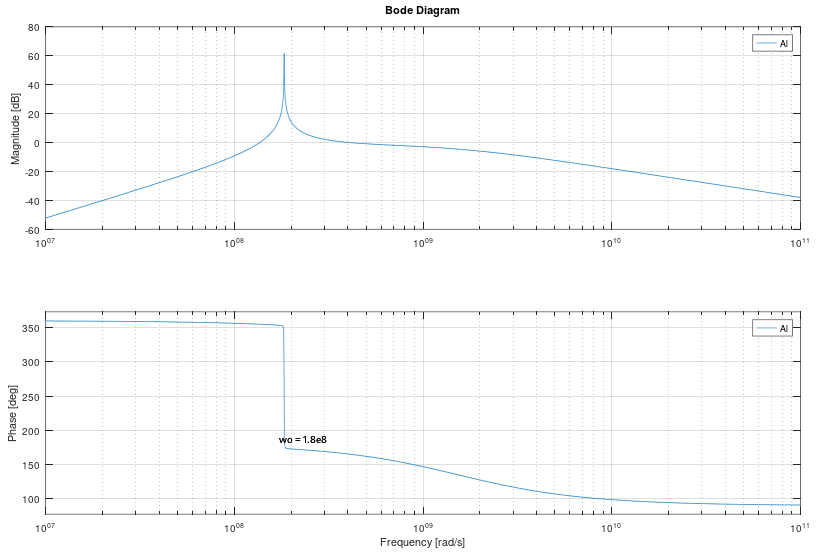
\includegraphics[scale=1, width=.8\textwidth]{bode_tx}
    \caption{Diagrama de Bode de la ganancia en lazo abierto del oscilador $A_l$ para frecuencias intermedias}
    \label{fig:bode_tx}
\end{figure}
En el diagrama de Bode de la figura \ref{fig:bode_tx}, se obtiene una frecuencia angular $\omega_0 = \SI{1.8e8}{\radian\per\second}$, por lo que se obtiene una frecuencia de resonancia de:
\begin{equation}
   f_0 = \frac{\omega_0}{2\cdot\pi} = \SI{28.65}{\mega\hertz}
\end{equation}
\paragraph{}
La obtenci\'on del diagrama de Bode se ha conseguido por medio del programa de c\'alculo computacional Octave REFERENCIA

\paragraph{} la señal digital de inicio o corte es producida por el microcontrolador Atmega328p, y se desarrollará en el correspondiente apartado CITAR. El transistor PNP es utilizado como conmutador.

\paragraph{Antena} CALCULOS DEL TRANSFORMADOR, EXPLICAR EL CONDENSADOR ES PARA QUE AL TOCARLA NO PASE NADA.
simulacion de potencia disipada por la antena?
\paragraph{Resultado de la Simulaci\'on} SIMULACION LTSPICE
son 3 capturas una la de la oscilacion con las medidas de frecuencia.
una general con varios ciclos de digitalin.
otra del flanco de subida y bajada de digitalin con vout y vbe viendo como se corta el transistor.
\paragraph{Resultado de la pr\'actica} CAPTURA DEL OSCILOSCOPIO Y MEDIDA DE CORRIENTE
\paragraph{}
Explicacion de la relevancia de una buena antena en transmision, el cuerpo humano como antena(bibliografia)

% \paragraph{Modulaci\'on de los canales mediante NE555}
% \paragraph{}
% La estrategia para la modulaci\'on reside en concepto de NE555 es un chip, el cual, configurado adecuadamente puede trabajar como un astable. Adem\'as, la frecuencia de oscilación del astable puede ser variada en función de los elementos de configuración. La idea es utilizar la señal proporcionada por el chip para cortar el oscilador según la frecuencia del NE555, realizando una mezcla de ambas señales y dando lugar a la señal modulada ASK. La mezcla se realiza por medio del transistor Q2 PNP, el cual trabaja en corte y saturación.
% \paragraph{}
% La configuraci\'on de astable para el chip NE555 viene dada en la datasheet del mismo, por lo que se sigue el modelo de esta configuraci\'on. El chip soporta un rango de tensiones de alimentaci\'on $4.5 < V_{CC} < 16$ \unit{\volt}, por lo que se ajusta a las condiciones del trabajo. Se realiza el diseño y el valor de los componentes siguiendo las siguientes ecuaciones proporcionadas por la hoja de datos:
% 
% \begin{align} 
%    \label{eq:freq}
%    Freq &= \frac{1.44}{(R_A + 2 \cdot R_B) \cdot C} \\
%    \label{eq:duty}
%    Duty &= \frac{1.44}{(R_A + 2 \cdot R_B)}
% \end{align}
% 
% Se requiere un ciclo de trabajo de aproximadamente $Duty \approx 0.5$ por lo que $R_B >> R_A$. La frecuencias de la onda cuadrada moduladora son de \SI{15}{\kilo\hertz} y \SI{3}{\kilo\hertz} para distintos valores de $R_B$. Estas frecuencias son alternadas mediante dos pulsadores los cuales conectan los dos distintos valores de $R_B$ al circuito tras ser accionados, generando as\'i dos distintos canales digitales. Cabe mencionar que $R_A$ no puede ser arbitrariamente pequeña, pues el el esquema eléctrico del chip que proporciona el fabricante, $R_A$ se conecta como resistencia de colector del transistor de \textit{DISCH}. Hacer $R_A$ más pequeño incurre en mayor consumo del chip en cada semiciclo.
% \paragraph{}
% Las frecuencias de modulación se eligen teniendo en cuenta: la facilidad de filtrado con respecto a las bajas frecuencias, los valores de $R_B$ y $R_A$, y la frecuencia de muestreo del ADC en el decodificador digital. Teniendo en cuenta estos parámetros, se calculan $R_A$ y $R_B$ con las ecuaciones.
% \paragraph{}
% En primer lugar, se selecciona $R_A$ para obtener un consumo razonable de descarga siguiendo la ecuaci\'on $I_{Disch} = \frac{V_{CC}-0.2}{R_A}$, un valor de $R_A = \SI{500}{\ohm}$ da lugar a $I_{Disch} = \SI{17.6}{\milli\ampere}$, lo cual es aceptable. En segundo lugar se debe fijar el ciclo de trabajo, si se hace $R_B = 10 \cdot R_A$ es una aproximaci\'on suficiente, ya que, mediante la ecuaci\'on \ref{eq:duty} queda $Duty = 0.476 \approx 0.5$. Por \'ultimo se fijan las frecuencias de modulaci\'on mediante la ecuaci\'on \ref{eq:freq}, lo cual nos fija un valor de $C$. Al tener dos diferentes canales con dos valores de frecuencia y $R_B$, se obtiene el siguiente sistema de ecuaciones para obtener el valor de $C$:
% \begin{align*} 
%    Freq_1 &= \frac{1.44}{(R_A + 2 \cdot R_{B1}) \cdot C} \\
%    Freq_2 &= \frac{1.44}{(R_A + 2 \cdot R_{B2}) \cdot C} \\
% \end{align*}
% 
% siendo  $Freq_1= \SI{15}{\kilo\hertz}$ $Freq_2=\SI{3}{\kilo\hertz}$ $R_{B1}=\SI{10}{\kilo\ohm}$ $R_{B2}=\SI{5}{\kilo\ohm}$, el valor de $C$ como resultado es $C \approx \SI{6.8}{\nano\farad}$




\newpage
   \subsubsection{Diseño de la parte anal\'ogica de RF del receptor}
   \paragraph{}
%explicar separacion de partes entre oscilador y quench signal
El diseño del receptor se ha de separar en tres partes diferenciadas.
En primer lugar, la parte correspondiente al punto de operación del transistor, donde se trabaja con la componente DC.
En segundo lugar, se desarrolla la parte de RF correspondiente al oscilador, el cual define la frecuencia de trabajo. 
Por último, la parte correspondiente a la \textit{quench-signal}, encargada de gestionar el paro y arranque de la oscilación. Esta parte trabaja a una frecuencia intermedia que puede diferenciarse de la parte de RF y de la componente DC.

El esquema completo del receptor se expone en la figura \ref{fig:rx}.
\begin{figure}[h]
    \centering
    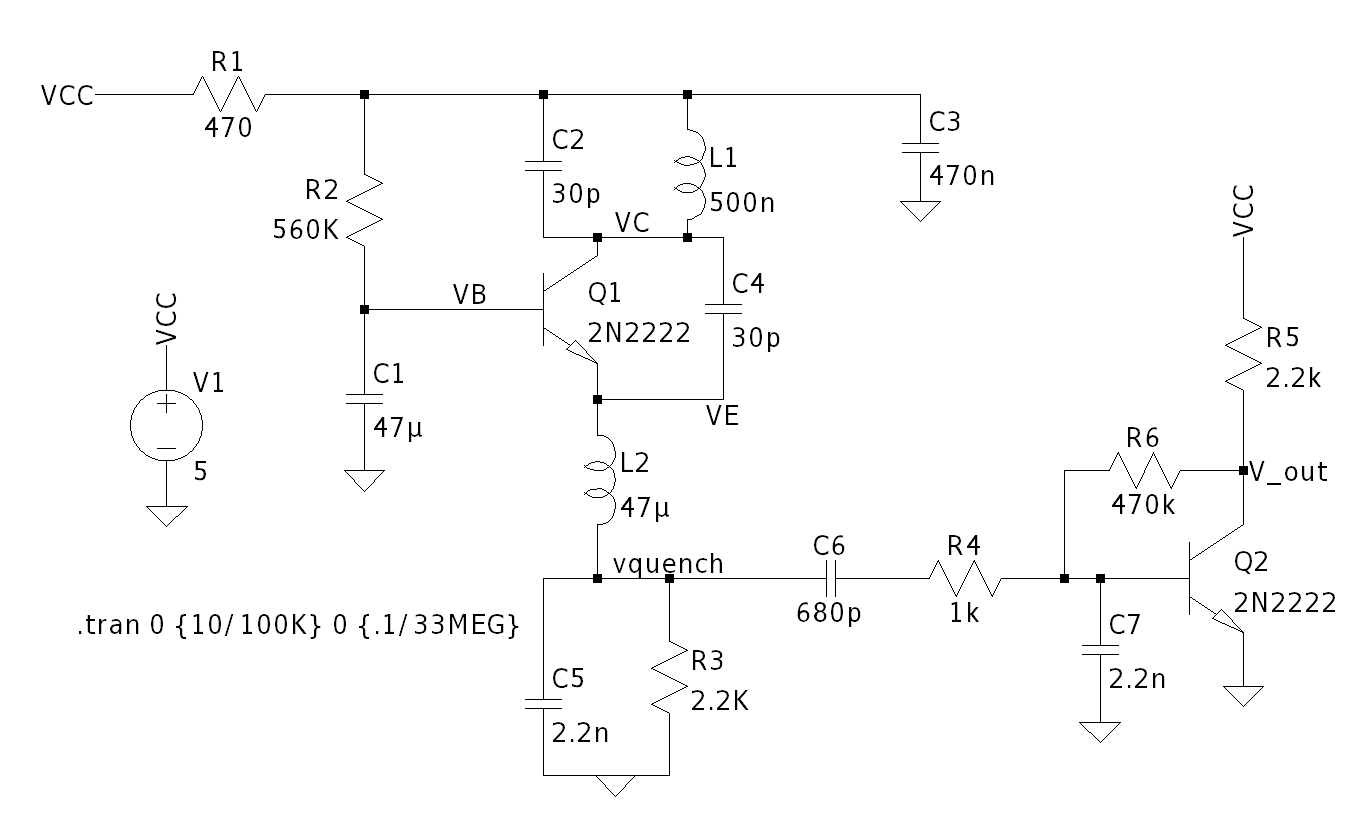
\includegraphics[scale=1, width=1\textwidth]{receptor}
    \caption{Esquema el\'ectrico del receptor}
    \label{fig:rx}
\end{figure}

\paragraph{Polarización} %EXPLICAR PORQUE ESE PUNTO DE OPERACION (MENOR RUIDO POSIBLE, MENOR CONSUMO DE POTENCIA)
En este caso, la estrategia para fijar el punto de operación es ligeramente distinta a como se diseña en el transmisor. 
El transistor debe trabajar en zona activa directa, por lo que se fijará $V_{CE} = \frac{V_{CC}}{2}$ para garantizar el mayor rango de linealidad posible.
También se elige una $I_C = \SI{1}{\milli\ampere}$, en este caso para que el transistor trabaje introduciendo el mínimo ruido posible.
Este hecho es importante, pues cuando el receptor se encuentran en la etapa de inicio de oscilación, un bajo nivel de ruido ayuda a aumentar la sensibilidad del receptor. Esto es debido a que la suma mínima de todos los ruidos generados por un transistor se encuentra en este rango de corriente de colector\footnote{Horowitz, P., \& Hill, W. (2015). \textit{The Art of Electronics} (Capítulo 8: Low Noise Techniques). Cambridge University Press.}.
Cabe recalcar que la estructura del circuito de polarización posee una estructura de realimentación de colector. Esta estructura, provoca una realimentación negativa que fija el punto de operación de manera más independiente a los parámetros característicos del transistor. Esta realimentación negativa debe eliminarse en corriente alterna para provocar la oscilación. La estrategia para eliminarla se verá en el apartado de pequeña señal.
\paragraph{}
Se realizan los cálculos para estimar los valores de las resistencias de polarización en función de los valores anteriormente fijados.
HACER LOS CALCULOS

\paragraph{Parte oscilador RF} IGUAL QUE EN TRANSMISOR. SMALL-SIGNAL ETC 
La estructura del oscilador en el receptor es idéntica al transmisor. Para evitar la realimentación negativa provocada por la parte de polarización se coloca el condensador $C_3 = \SI{470}{\nano\farad}$, este valor es suficiente para que su impedancia para la frecuencia de RF suponga un cortocircuito a tierra. La inclusión de este condensador es imprescindible para que el circuito funcione. 
\paragraph{Modelo en pequeña señal:} Debido a que el diseño es estructuralmente igual que en el transmisor, los cálculos serán idénticos sustituyendo los valores correspondientes.
Se incluyen los valores característicos junto a las ecuaciones de interés.
En función de los valores del punto de operación obtenido, se calculan los parámetros híbridos para el receptor.

\begin{equation}
   \label{eq:result_pol1}
V_{AF} = \frac{I_{Cdata}}{h_{OEdata}} =\frac{\SI{1}{\milli\ampere}}{\SI{6}{\micro\siemens}} =  \SI{50}{\volt} 
\end{equation}
\begin{equation}
   \label{eq:result_pol2}
%\[
\begin{array}{rl} 
      \begin{array}{l}
	 h_{ib} =  \SI{8.4}{\ohm} \\
	 h_{fb} =  -0.99
      \end{array}
      &
      \begin{array}{l}
	 h_{rb} =  0.014 \\
	 h_{ob} =  \SI{6}{\micro\siemens}
      \end{array}
\end{array}
%\]
\end{equation}

\paragraph{}
El modelo en pequeña señal para las frecuencias de RF es sustancialmente igual a la parte del transmisor (apartado \ref{des_tx.tex}). En la figura \ref{fig:ss_rx}, se muestra el modelo del receptor en pequeña señal para las frecuencias de RF. $L_2$ tiene una impedancia suficientemente grande como para considerarla circuito abierto. El objetivo del modelo es la obtención de una expresión para la frecuencia de resonancia.

\begin{figure}[h]
    \centering
    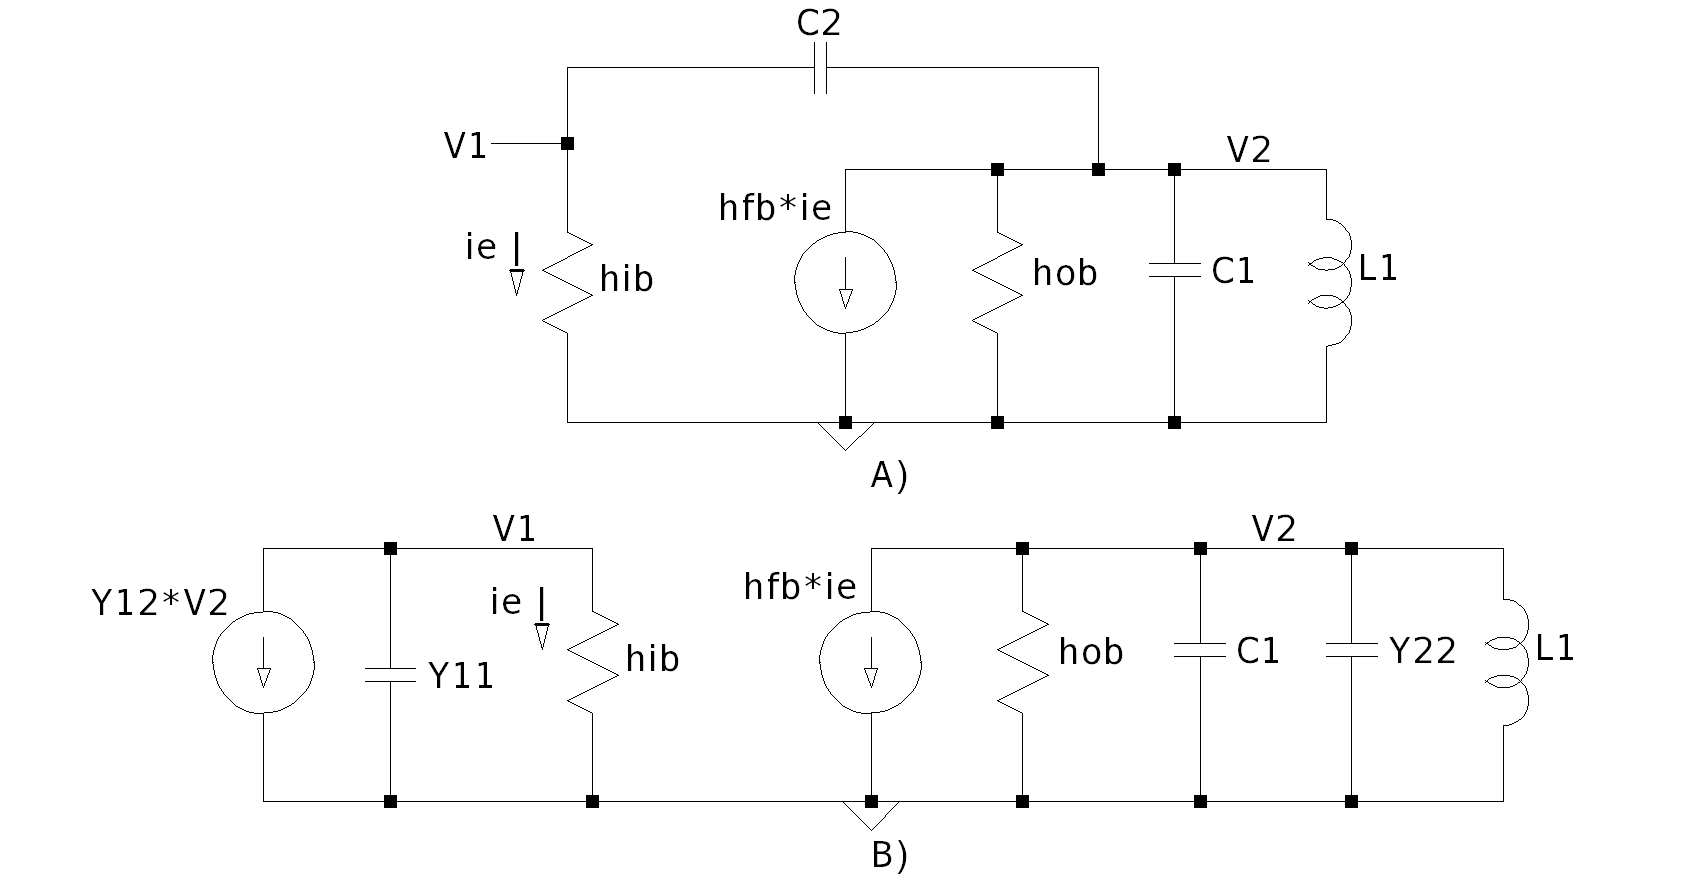
\includegraphics[scale=1, width=.8\textwidth]{small_signal_rx}
    \caption{A) Modelo en pequeña señal del bucle de oscilación para frecuencias de RF B) Modelo en pequeña señal del oscilador sustituyendo el condensador de realimentación $C_2$ por su equivalente en parámetros $Y$}
    \label{fig:ss_rx}
\end{figure}

%FALTA FUNCION DE TRANSFERENCIA IGUAL QUE TX Y CALCULO DE FREQ RESONANCIA IGUAL QUE TX. RAPIDAMENTE. DECIR QUE SE ANADE CONDENSADOR VARIABLE PARA SINTONIZAR ELUDIENDO LAS DISCREPANCIAS REALES DEL CIRCUITO.
\paragraph{}
Debido a la dualidad con respecto al tx, la expresión de la función de transferencia de lazo cerrado es idéntica al transmisor. La expresi\'on de la funci\'on de transferencia se muestra a continuaci\'on:

\begin{equation}
   \label{eq:Al_tx}
   A_l = \frac{h_{fb} \cdot C_1 \cdot s^2}{ \left( C_2+C_1 \right) \left( s \cdot h_{ib} \cdot C_2 + 1\right) \left( s^2 + s \cdot \frac{h_{ob}}{C_1 + C_2} + \frac{1}{(C_1 + C_2)\cdot L_1}\right) }
\end{equation}

\paragraph{}
Se obtiene la frecuencia de resonancia como: $$\omega_0^2 = \frac{1}{L_1 \cdot (C_1 + C_2)}$$
$$ f_0 = \frac{1}{2 \cdot \pi \cdot \sqrt{L_1 \cdot (C_1 + C_2)}} $$
\paragraph{}
Se obtiene el valor de la inductancia con la siguiente expresi\'on explicada en el apartado \ref{sec:des_tx}:
\begin{equation}
	\label{eq:inductance}
PONER DEL OCTAVE
\end{equation}
$$ L_1 = \SI{500}{\nano\henry} $$


\paragraph{\textit{Quench-signal}} %AISLAR CIRCUITO, REALIZAR C\'ALCULOS, L(CHOKE) R Y C
\paragraph{}
En este caso, al contrario que en el receptor, la bobina de RFC no podrá ser arbitrariamente grande, pues debe permitir el paso de la frecuencia de \textit{quench} pero no de la señal de RF.
%El par RC provocan la oscilación de paro y marcha del circuito, pues al realizar los cálculos, se observa que sus valores fijan el coeficiente de amortiguación del sistema. 
%i think i have now understood, the value of L2 is critical because it needs to be as large as possible to be a high impedance for rf, but an intermediate impedance to quench. This quench frequency will be always the higher possible that could be amplified in the possitive loop and at the same time can pass in the low pass filter no?
\paragraph{}
En primer lugar, es necesario una explicación analítica del fenómeno para facilitar el entendimiento antes de realizar los cálculos de interés.
El transistor trabaja en configuración de base común. Esto implica que la tensión de base $V_B$ es fija, mientras que $V_E$ varía en el tiempo cortando y activando el transistor. Para un mejor entendimiento, se habla de $V_E$ como $V_{quench}$ indistintamente, pues $V_{quench}$ es $V_E$ tras el filtro paso bajo, eliminando visualmente la componente RF. La componente de baja frecuencia es quien corta el transistor de forma general. En la figura \ref{fig:quench-explain} se observa de forma gráfica la explicación dada a continuación.
\paragraph{}
Partiendo de una tensión $V_B - V_{quench} \approx \SI{0.7}{\volt}$, la oscilación comienza a generarse.
%Se toma como referencia $V_{quench}$ y no $V_E$ debido a que $V_E$ proporciona información tanto de las frecuencias de RF como las de frecuencia de quench, mientras que $V_{quench}$ proporciona la información de las frecuencias de interés por actuar como filtro paso bajo. 
%Mientras que la frecuencia de RF evidententemente satura y corta el transistor en numerosos ciclos por segundo, quien importa es quien corta la oscilación. 
A medida que la oscilación, al encontrarse dentro de un bucle de realimentación positiva, va incrementando su amplitud, la tensión media $V_{quench}$ también aumenta. En el momento que $V_{quench}$ aumenta de forma que $V_B - V_{quench} < \SI{0.7}{\volt}$, el transistor se corta, matando la oscilación y provocando que la tensión $V_{quench}$ descienda, volviendo de esta forma a completar el ciclo.
\paragraph{}
Para calcular la frecuencia de \textit{quench}, se debe tener en cuenta el filtro paso bajo formado por $L_2, C_5$ y $R_3$. 
Se calcula la función de transferencia del conjunto de estos tres elementos, al cual se le llamará cicuito de \textit{quench}.
Se pretende obtener la expresión para la función de transferencia de $H(s) = \frac{i_{L_2}}{v_i}$. 

\begin{align*} 
   v_i &= i_{L_2} \cdot ( Z_1 + Z_2 ) \\
   Z_1 &= s\cdot L_2 + r_s \\
   Z_2 &= \frac{R_3}{s \cdot R_3 \cdot C_5} \\
   \frac{i_{L_2}}{v_i} &= \frac{1}{( Z_1 + Z_2 )} = \frac{(s\cdot R_3 \cdot C_5 + 1)}{rs \cdot (s\cdot R_3 \cdot C_5 + 1) + s \cdot L_2 \cdot(s\cdot R_3 \cdot C_5 + 1) + R_3 } \\
\end{align*}

\begin{equation}
   \label{eq:Al_tx}
   H(s) = \frac{i_{L_2}}{v_i} = \frac{(s\cdot R_3 \cdot C_5 + 1)}{R_3 \cdot ( s\cdot r_s \cdot C_5 + s^2 \cdot L_2 \cdot C_5 + 1)}
\end{equation}
\paragraph{}
Se calcula la frecuencia de resonancia como $$\omega_0^2 = \frac{1}{L_2 \cdot C_5}$$
$$ f_0 = \frac{1}{2 \cdot \pi \cdot \sqrt{L_2 \cdot C_5}} = \SI{495}{\kilo\hertz} $$
%pero no en este caso la frecuencia de quench no se corresponde con la frecuencia de corte del filtro, ya que, el condensador no se descarga completamente en sus ciclos pues depende del transistor. 
\paragraph{}
En la figura \ref{fig:quench-explain}, se muestra por un lado, a la izquierda, la respuesta en frequencia del circuito de \textit{quench}, compuesto por: $L_2, R_3$ y $C_5$ en el esquemático del transmisor (figura \ref{fig:rx}). La respuesta en frecuencia es simulada para varios valores de $L_2$, y se indica con cursores. En el caso el caso de $L_2 = \SI{47}{\micro\henry}$, el valor de su frecuencia de corte es $f_c = \SI{483}{\kilo\hertz}$. 
\paragraph{}
Por otro lado, a la derecha, se muestra la simulación en función del tiempo del receptor. Se hace hincapié en la corriente de $L_2$. Esta está cursorizada de forma aproximada al valor que debería tener si a través de la bobina pudiera conducir corriente negativa, siendo este valor igual que el de la frecuencia de corte en la simulaci\'on en frecuencia.
La corriente de la inductancia $L_2$ no puede ser negativa, pues en este sentido de circulación la unión PN base emisor se encuentra inversamente polarizada y el condensador de realimentación tiene alta impedancia para frecuencias bajas. 

\begin{figure}[h!]
    \centering
    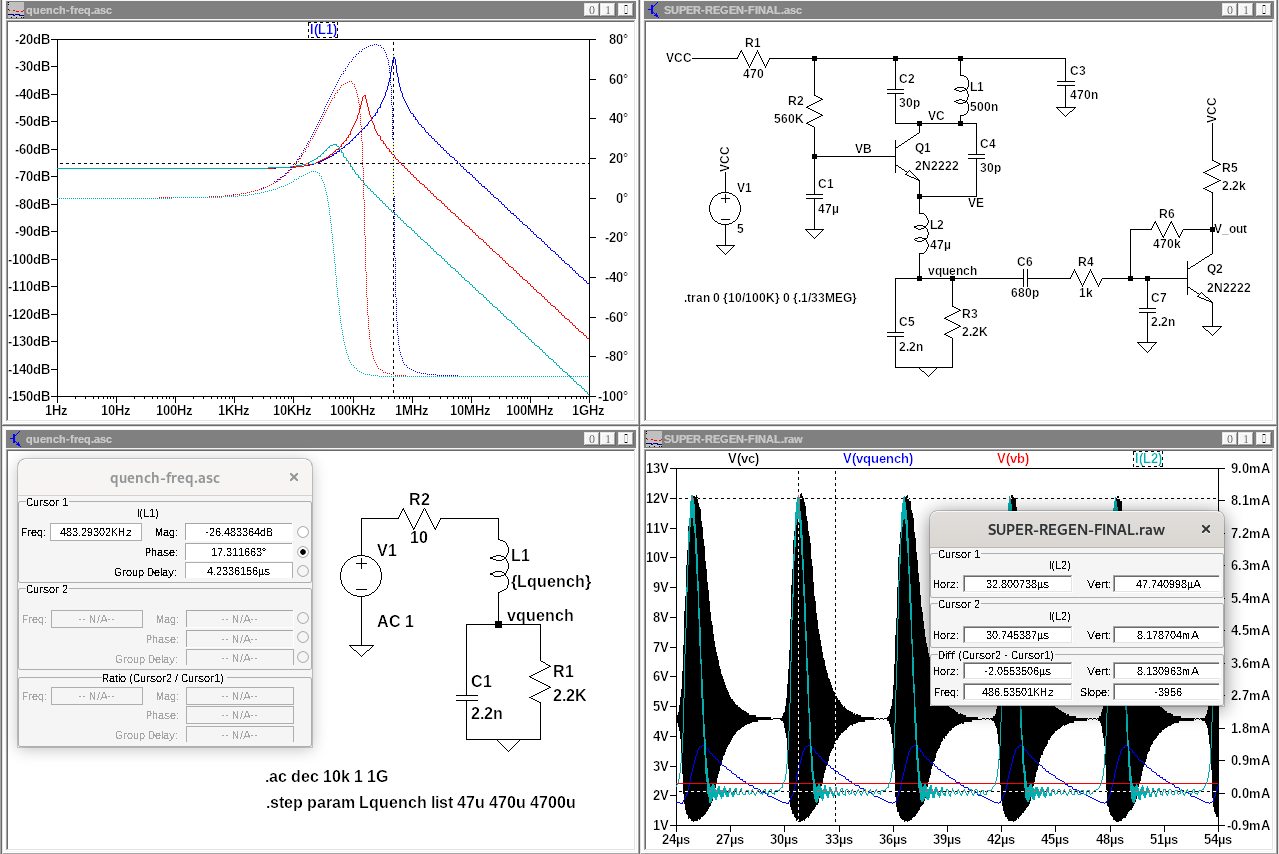
\includegraphics[scale=1, width=1\textwidth]{quench-explain}
    \caption{quench explain}
    \label{fig:quench-explain}
\end{figure}

\paragraph{}
%REF Tipler pag 869. descarga condensador
En cualquier caso, la frecuencia real de \textit{quench} no es la calculada en la ecuacion \ref{eq:Al_tx}, sino que la señal de \textit{quench} se genera como se muestra en la figura \ref{fig:quench-explain}. 
En el momento que $i_{L_2} = 0$, la tensión en $V_{quench}$ se descarga a trav\'es de $R_3$, siguiendo $\tau$ de $C_3$ y $R_3$ hasta que $V_B - V_{quench} < 0.7$, reiniciando el ciclo.
El tiempo de subida depende tanto del tiempo que tarda en reconstruirse la oscilaci\'on como de la constante de elongación del sistema de la ecuación REF. Esta constante viene dada por $r_s$ y $C_5$ EXPRESION y define $v_{oi}$.
Se calcula aproximadamente la frecuencia de \textit{quench} siguiendo los valores de la figura \ref{fig:quench-explain}. 
\begin{align*} 
   &i_{C_5} + i_{R_3} = 0 \\
   &C_5 \cdot \frac{dv_0(t)}{dt} + \frac{v_0(t)}{R_3} = 0 \\
   &\int_{v_{0i}}^{v_0(t)} \frac{1}{v_0(t)} \, dv_0(t) = \int_{0}^{t} \frac{-1}{R_3 \cdot C_5} \, dt \\
\end{align*}

\begin{equation}
   \label{eq:des_rx-rc}
   ln \left( \frac{v_0(t)}{v_{oi}} \right) = \frac{-t}{R_3 \cdot C_5}
\end{equation}
\begin{equation}
%   \label{eq:Al_tx}
   \frac{v_0(t)}{v_{oi}} = e^{\left( \frac{-t}{R_3 \cdot C_5} \right)}
\end{equation}

\paragraph{}
Se usa \ref{eq:des_rx-rc} para calcular el tiempo de descarga con los valores de la figura \ref{fig:quench-explain}.
$$ t_{disch} = \SI{3.62}{\micro\second} $$
A este tiempo, se le debe sumar el tiempo de subida que viene dado por el tiempo de construcción de la oscilación junto con el tiempo de subida del sistema del circuito \textit{quench}.
Este tiempo, se aproximar\'a como $t_{rise} \approx t_{disch}$. Por lo que $$t_{quench} \approx 2 \cdot t_{disch}$$ y por tanto $$f_{quench} = \frac{1}{t_{quench}}  = \SI{138}{\kilo\hertz} $$
\paragraph{}
Empíricamente, esta frecuencia resulta en $f_{quench} = \SI{67}{\kilo\hertz}$. Esto es debido a que los valores en la simulación difieren bastante de la realidad, pero no las formas de onda. El ajuste de la frecuencia de \textit{quench} empírica se realiza probando distintos valores de $C_5$ y $L_2$, pues $R_3$ se fija al polarizar el transistor.

\paragraph{Resultado de la simulaci\'on} 
%Se muestran las medidas simuladas de tension de mayor inter\'es con la nomenclatura de la figura FIG RF
%captura de oscilacion de rf, v en rc y vout
%captura con senal de entrada vout cambia de frecuencia
\paragraph{}
En el apartado de simulación, se trata de obtener una representación gráfica de lo desarrollado anteriormente sobre el receptor. Por ello, en la figura REF se observan los puntos de interés del circuito como son $V_C$, $V_{quench}$ y $V_{B}$, además de añadir la diferencia$V_B - V_{quench}$ como $V(B,quench)$. Estas cuatro medidas son suficientes para entender el ciclo de paro y marcha del transistor.
\paragraph{}
Como se puede observar en la figura \ref{fig:simrx_zoom}, a medida que se construye la oscilación, el valor medio de la tensión de $V_{C}$ (es decir $V_{quench}$) aumenta hasta que, finalmente, la diferencia $V_B - V_{quench} < \SI{.7}{\volt}$ hace desaparecer la oscilaci\'on. Este corte provoca que el valor medio de $V_C$ descienda, y por tanto $V_{quench}$, provocando finalmente que la diferencia $V_B - V_{quench} > \SI{.7}{\volt}$, reactivando al transistor y reiniciando el ciclo de oscilaci\'on.

\begin{figure}[h!]
    \centering
    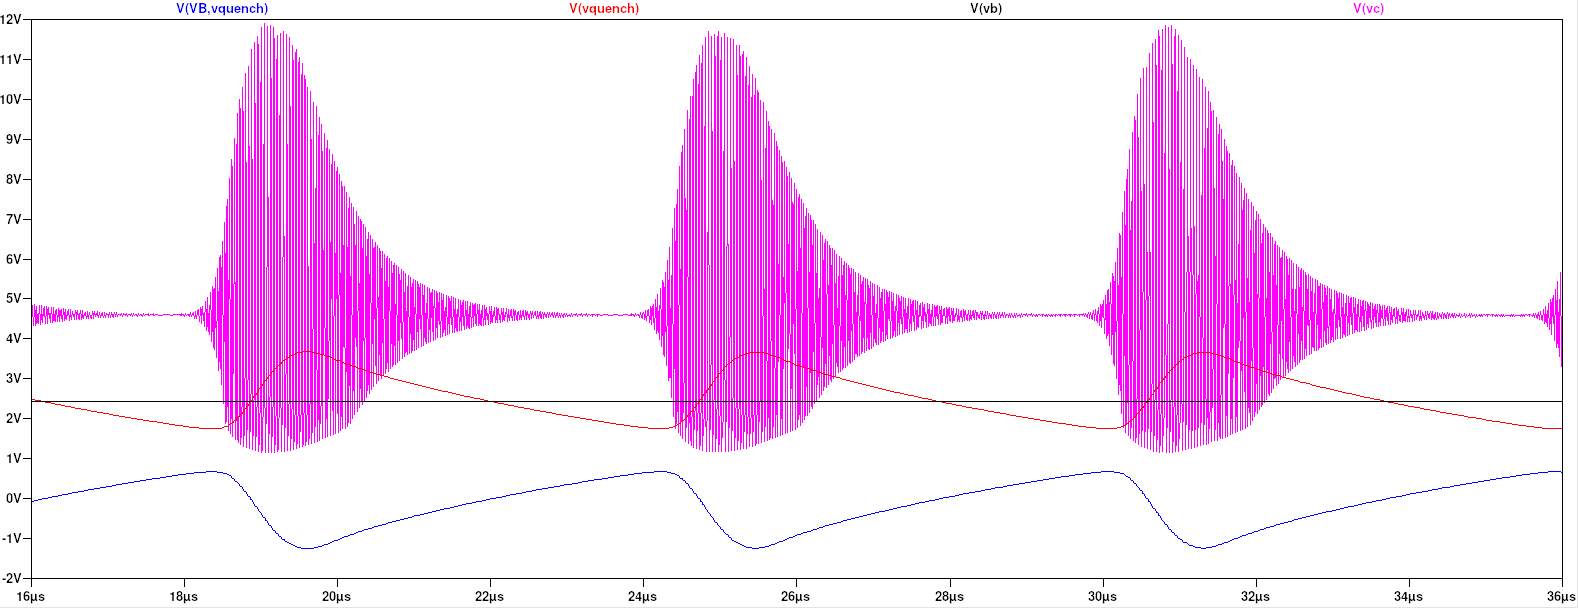
\includegraphics[scale=.8, width=.8\textwidth]{simrx_zoom}
    \caption{Simulación de puntos de interés en varios ciclos ampliados}
    \label{fig:simrx_zoom}
\end{figure}

\paragraph{}
Se añade también, en la figura \ref{fig:simrx_vout}, la forma de onda de la tensión de salida $V_{out}$, que es la señal de entrada al microcontrolador atmega328p, el cual se encargará de demodular la señal. Esta señal debe ser una señal digital entre \SI{0}{\volt} y \SI{5}{\volt}.
\begin{figure}[h!]
    \centering
    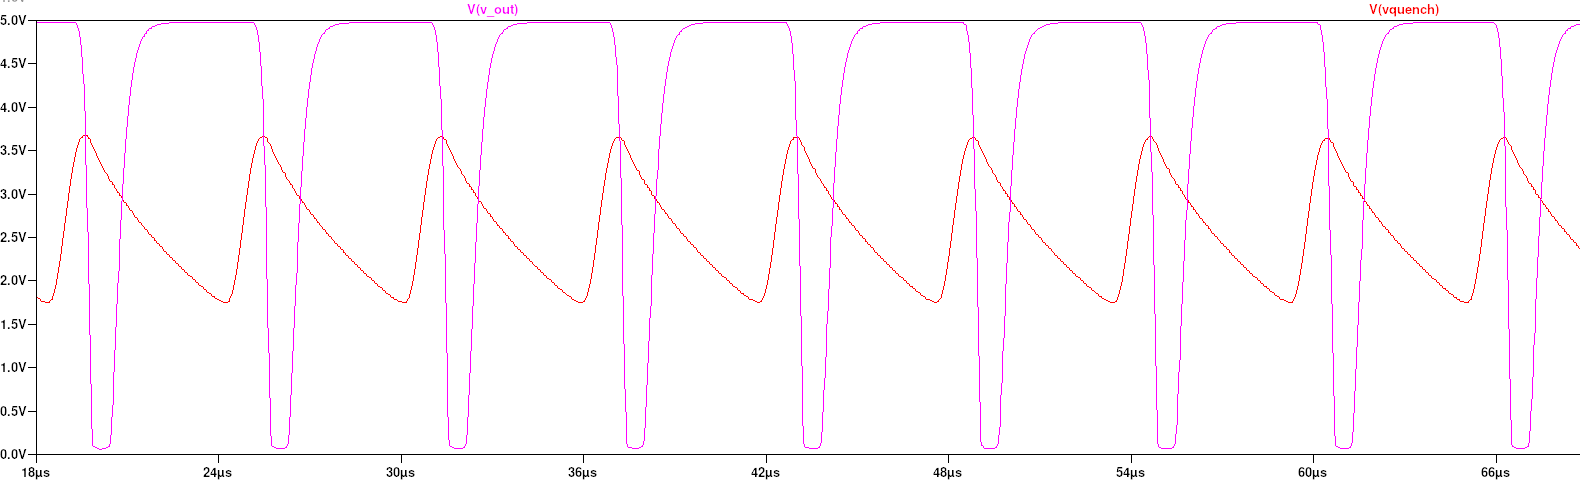
\includegraphics[scale=.8, width=.8\textwidth]{simrx_vout}
    \caption{Simulación de $V_{out}$ junto a $V_{quench}$}
    \label{fig:simrx_vout}
\end{figure}

\paragraph{Resultado práctico} 
\paragraph{}
En este caso se muestran las medidas tomadas en el apartado de simulaci\'on, esta vez tomadas en el circuito real. Las medidas se toman usando un osciloscopio. 
La configuración es la misma que en el en el apartado \ref{sec:des_tx} del transmisor. En este caso, al disponer de dos canales, se muestran en la figura \ref{fig:exp_vc_vquench} los puntos $V_{quench}$ (rojo) y $V_{C}$ (negro).

\begin{figure}[h!]
    \centering
    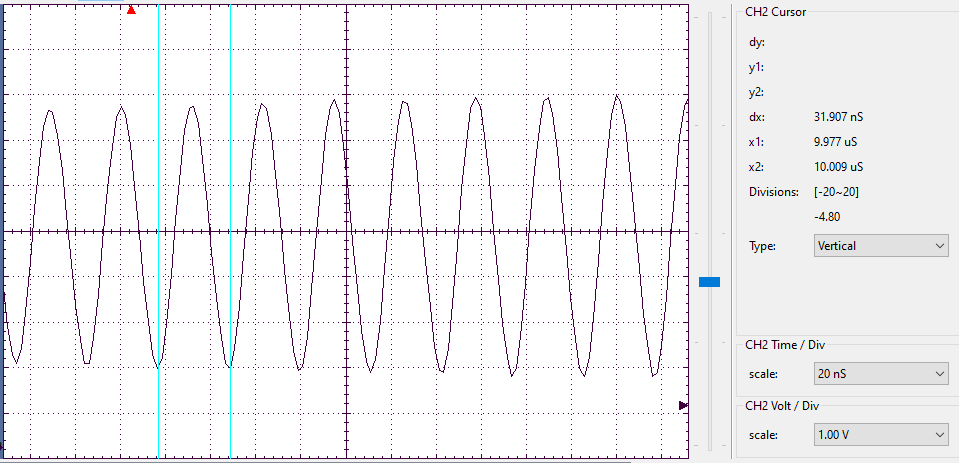
\includegraphics[scale=.7, width=.7\textwidth]{exp_work_freq.png}
    \caption{experimental de puntos de interés en varios ciclos ampliados}
    \label{fig:simrx_zoom}
\end{figure}
\begin{figure}[h!]
    \centering
    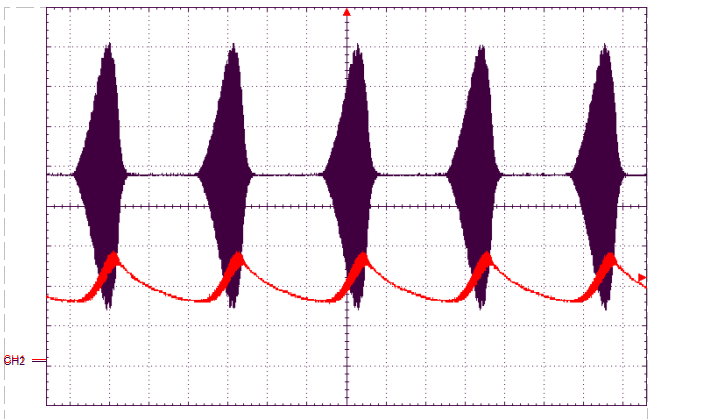
\includegraphics[scale=.7, width=.7\textwidth]{exp_quench+VC.PNG}
    \caption{Experimental $V_C$ (negro) y $V_{quench}$ rojo}
    \label{fig:exp_vc_vquench}
\end{figure}
\begin{figure}[h!]
    \centering
    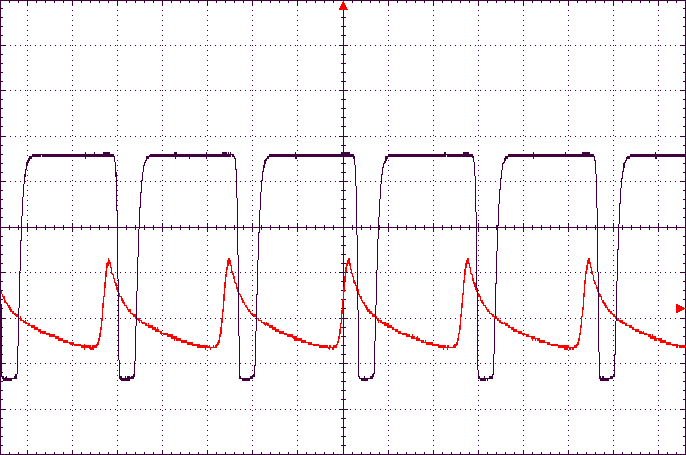
\includegraphics[scale=.7, width=.7\textwidth]{exp_quench+vout.png}
    \caption{experimental de puntos de interés en varios ciclos ampliados}
    \label{fig:simrx_zoom}
\end{figure}

% situacion en el circuito (imagen bloque) y partes, enumeracion partes
% explicacion recepcion directa amplificando senal de RF y demodulando con filtro, posteriormente etapa de smith triger que se 
% manda al microcontrolador y detecta el canal. 
% \subsubsection{sintonizaci\'on y etapa de par Darlington}
% El circuito sintonizado que consigue la sensibilidad necesaria para captar la señal modulada proviniente del transmisor se consigue mediante un filtro paso banda sintonizado a la frecuencia de portadora. La corriente en la bobina $L_1$ producida por el campo electromagnético recibido, se amplifica notablemente a trav\'es de la etapa darlington, la cual, se encuentra polarizada con un $V_{CE}$ suficientemente bajo como para provocar la saturaci\'on del transistor ante la m\'inima intensidad de corriente en su entrada.
% \paragraph{Polarizaci\'on:} el par darlington debe ser lo suficientemente sensible como para poder detectar la corriente inducida en la bobina de recepci\'on, por lo que $I_B \approx \SI{28}{\nano\ampere}$
% \paragraph{Modelo en pequeña señal:} El objetivo de este apartado es el cálculo de la ganancia de la corriente de entrada con respecto a la tensión de salida de la etapa, y su impedancia de salida
% \subsubsection{Etapa en colector com\'un}
% Esta etapa actúa como un adaptador de impedancias de tal forma que la tensión de salida de la etapa darlington ataque a una impedancia de entrada alta para evitar pérdidas, mientras que la impedancia de salida de la etapa en colector común es baja y de ganancia en tensión similar a la unidad. A esta configuración se la conoce como \textit{"voltage buffer"}.
% \paragraph{Polarizaci\'on:} Se debe fijar una corriente de base del orden de la corriente que pueda proporcionar la etapa anterior, unos \SI{30}{\micro\ampere}. De forma an\'aloga a los anteriores apartados, se calcula el punto de operaci\'on para los valores del esquem\'atico, figura \ref{}
% \subsubsection{Amplificador de tensi\'on y filtro paso bajo}
% \subsubsection{comparador Smith triger}
% \subsubsection{Demodulaci\'on digital}
% demodulaci\'on digital a tr\'aves del microcontrolador se expondra en la sección 


\newpage
   \subsection{Parte digital}
   \paragraph{}
Para establecer un canal de comunicación de datos digital, se utilizan dos microcontroladores para la codificación y la demodulación de los mismos. En este caso, el modelo de microcontrolador utlizado es el mismo en ambos dispositivos, el Atmega328p, pero con distintos programas dependiendo de si se utiliza en el transmisor o receptor.

\paragraph{Configuraci\'on del entorno de trabajo}
\paragraph{}
El microcontrolador se programa por medio de un proyecto escrito en C, utilizando como base la librería \textit{avr-libc}\footnote{\textit{AVR Libc User Manual}. (s.f.). Recuperado de https://www.nongnu.org/avr-libc/user-manual/}.
Para ello, se trabaja con las herramientas que permiten la compilación de este lenguaje a un archivo ejecutable entendible para la plataforma de AVR.
\paragraph{}
En primer lugar, es necesario compilar el programa en c\'odigo fuente a un archivo binario para la plataforma objetivo, para ello se usar\'a el compilador \textit{avr-gcc}. Este archivo binario generado no puede ser grabado directamente a la flash del microcontrolador, sino que se necesita la traducción a código hexadecimal del mismo. Para ello, se utiliza el programa \textit{avr-objcopy}. 
Finalmente, el programa es grabado en la flash. Este proceso se realiza de la siguiente forma: el archivo hexadecimal debe ser grabado en el microcontrolador configurando el microcontrolador en modo programaci\'on de la flash y transfiriendo el programa por medio del protocolo ISP. 
Para ello se har\'a uso de un programador software, \textit{avrdude}, y un programador hardware que traduzca el protocolo USB del ordenador de trabajo a ISP para ser grabado en la memoria del microcontrolador objetivo. 
\paragraph{}
En este proyecto se utiliza como programador un microcontrolador Atmega2560 en una placa Mega2560 R3. 
La placa Mega2560 R3 se programa con un software que permita el proceso de traducción anteriormente descrito. Este software se ofrece oficialmente desde la p\'agina web de Arduino\footnote{\textit{https://docs.arduino.cc/built-in-examples/arduino-isp/ArduinoISP/}}.
Para automatizar todo el proceso de compilaci\'on y programaci\'on del microcontrolador objetivo, se hace uso de la herramienta \textit{make}. A continuaci\'on, se muestra un archivo \textit{Makefile} utilizado para clarificar el proceso anteriormente descrito:

\lstinputlisting[language=make]{/home/jose/Documents/tfg2/digital/gpio_signaldriven/v6_final/Makefile}

\paragraph{}
Es importante destacar que los microcontroladores AVR poseen unos registros especiales denominados \textit{fuses}.
Estos registros poseen configuraciones cr\'iticas para el microcontrolador como la fuente que se utiliza como reloj de CPU. Esta puede ser configurada como externa o interna, a diferentes frecuencias. Por defecto de fábrica, viene configurado usando el oscilador interno de \SI{8}{\mega\hertz}, con un prescaler de 8, resultando en $F_{CPU} = \SI{1}{\mega\hertz}$.
\paragraph{}
En la pr\'actica, se tuvo que modificar uno de los \textit{fuses}, concretamente, el \textit{lfuse}. El prop\'osito final era cambiar la frecuencia de reloj de la CPU modificando el bit de prescaler.
Para lidiar con los aspectos referentes a los \textit{fuses}, se crearon dos guiones \textit{Bash}: \textit{fuses.sh} y \textit{write\_fuses.sh}, para leer y escribir respectivamente en ellos. A continuaci\'on se muestra \textit{fuses.sh}:
\lstinputlisting[language=make]{/home/jose/Documents/tfg2/digital/fuses.sh}

\paragraph{}
Por último, cabe mencionar que los archivos de código fuente junto a todo el proyecto han sido desarrollados mediante el programa de control de versiones \textit{git}. 
Los repositorios tanto del proyecto como del código fuente se encuentran en GitHub\footnote{\textit{https://github.com/josegu05/tfg2}}.


   \subsubsection{Diseño del demodulador digital para la recepci\'on}
   \paragraph{} El objetivo del microcontrolador en la parte de recepción tiene dos funciones. Implementar un contador de frecuencia que identifique las variaciones recibidas por el m\'odulo de RF correspondientes a los diferentes s\'imbolos digitales, de tal forma que sirva como demodulador. y además decodificar la señal digital recibida, identificando la orden concreta transmitida por el transmisor.

\paragraph{Contador de frecuencia} 
\paragraph{}
Esta parte se implementa por medio de dos timers/counters incorporados en el SOC del Atmega328p. La configuraci\'on y uso de estos dispositivos se encuentra en la hoja de datos del microcontrolador (REF). La estrategia de implementación es la siguiente: mientras uno de los timers genera interrupciones periódicas en un intervalo de tiempo conocido. Durante el mismo espacio de tiempo, el segundo timer/counter, se encarga de detectar el número de flancos de subida o bajada producidos por la señal de salida codificada en FM del módulo de RF. Este proceso provoca un número de interrupciones variable en función de la frecuencia de la señal de entrada en un intervalo de tiempo conocido.

\paragraph{} Cada vez que el timer produzca su interrupción periódica, la rutina de tratamiento de interrupción (IRQ) se encargará de examinar el número de interrupciones producidas por el counter en ese lapso de tiempo y decidir si se ha recibido señal, en función del número de interrupciones del counter.

\paragraph{} Se hacen uso tanto del TIMER0 como del TIMER2, esto es debido a que poseen las mismas caracter\'isticas necesarias las cuales se encuentran expuestas en la hoja de datos. Existen a su vez, más timers/counters con características más complejas, pero no serán necesarias en este proyecto.
\paragraph{}
Se configura TIMER0 como temporizador, generando la interrupci\'on periódica necesaria conocida como \textit{gate}. mediante el registro de configuración propio del timer, se configura la frecuencia a la cual se genera esta interrupción peri\'odica. La rutina de tratamiento de interrupción ISR(TIMER0), incrementa una variable que permite conocer el n\'umero de veces que se genera la interrupci\'on.
% se encarga de comparar el número de interrupciones producidas por el counter, almacenadas en una variable global, y un número fijo umbral. Si el número de cuentas supera el umbral, la señal fue recibida, produciendo la demodulación digital. 
% PROBLEMAS ajuste tedioso muy dependiente de la frecuencia.
\paragraph{}
Por otro lado, TIMER2, se configura como contador, identificando los flancos de bajada de una señal externa introducida por el pin OSC2. La interrupción del TIMER2, se puede producir cada cierto número de flancos detectados. la rutina de tratamiento de interrupción ISR(TIMER2), incrementa la variable global de cuenta.

\paragraph{}
Finalmente, el objetivo del programa main(), es identificar la recepci\'on de señal y actuar en consecuencia.
Para ello, el programa actúa de la siguiente forma. 
En primer lugar, espera a que la interrupci\'on del temporizador \textit{gate} se haya activado el número de veces necesaria. Ambos contadores durante el periodo de espera se encuentran continuamente acturalizando.
Después se realiza una media aritmética dividiendo el número de flancos detectados por el contador entre el número de veces que \textit{gate} se activó.
En caso de que la media calculada supere la media calculada anteriormente, quiere decir que se ha detectado señal, por lo que el programa procede a actuar en consecuencia.
El programa implementa una máquina de estados en función del número de señales recibida.

\paragraph{Limitaciones}
\paragraph{}
Algunos problemas que surgieron a la hora de llevar a cabo esta realización fueron.
La velocidad de procesamiento de instrucciones debe ser decenas de veces más rápida que la frecuencia de entrada, \textit{quench-signal}. Siendo la rutina IRQ(TIMER2), del contador la función crítica.
En las primeras versiones del código recargaban mucho las rutinas de tratamiento de interrupción, escalando muy rápido este problema.
\paragraph{}
También, ha sido necesario introducir una función de startup(), ya que, en el momento que se conecta el circuito a la fuente de alimentación, la frecuencia de \textit{quench} tarda un tiempo en estabilizarse. La función startup(), asegura que la señal de \textit{quench} es estable.

%\paragraph{} Lo óptimo para que la identificación de las variaciones de frecuencia fuera lo más sensible posible sería que se provocara una interrupción con cada flanco de la señal de entrada y que la interrupción periódica del timer fuera lo más extensa posible, pero nos encontramos con varios limitantes: la frecuencia de reloj de CPU y su procesamiento de instrucciones y la velocidad de transmisión de datos (bps).
%\paragraph{} Para encontrar el límite se realiza un cálculo aproximado y posteriormete se ajustan los valores del programa con ayuda de un osciloscopio. El cálculo realizado es el siguiente: CALCULO.

\paragraph{Presentaci\'on del c\'odigo}
\paragraph{}
Todas las versiones de los c\'odigos, tanto del emisor como del receptor, se encuentran en el repositorio de GitHub\footnote{\textit{https://github.com/josegu05/tfg2}}. La versi\'on final del c\'odigo del receptor se muestra a continuaci\'on. El c\'odigo se presenta en dos columnas por hoja, el orden de lectura es el siguiente: primera columna, segunda columna, hoja siguiente.

\begin{multicols}{2}
\lstinputlisting[language=C]{/home/jose/Documents/tfg2/digital/receptor-8mhz-mean/main.c}
\end{multicols}

   \subsubsection{Diseño del codificador digital para la transmisi\'on}
   \label{sec:des_digital_tx}
   \paragraph{Introducción} El objetivo del microcontrolador en la parte de transmisión, codifica mensajes según los botones pulsados.
Consiste en tres pulsadores, donde cada cual codifica un símbolo diferente, para que el receptor actúe de manera distinta según el botón pulsado. El algoritmo de comunicación entre transmisor y receptor se realiza de manera asíncrona. Para diferenciar los símbolos digitales se ha de tener en cuenta el tipo de modulación ASK, donde el 1 implica recibir señal y el 0 no se ha recibido. 
Los relojes o timers encargados de la codificación y decodificación tanto en transmisión como en recepción, deben trabajar a la misma tasa de baudios para identificar correctamente los mensajes.

\paragraph{Configuraci\'on de reloj} 
\paragraph{Codificaci\'on de los mensajes} 
La codificación de los diferentes símbolos se desarrolla de forma que, los algoritmos de codificación y decodificación se realicen de la forma más sencilla y robusta posible, teniendo en cuenta el tipo de modulación ASK.
Es por eso que cada símbolo se representa por el número de unos lógicos transmitidos de forma que si quisieramos transmitir N símbolos, la serie de codificación sería:
\begin{table}[ht]
    \centering
    \begin{tabular}{|c|c|}
        \hline
        \textbf{Symbol} & \textbf{Codification} \\ 
        \hline
        1 & 0b1 \\ 
        2 & 0b11 \\ 
        3 & 0b111 \\ 
        N & 0b$111 \ldots 1 \cdot N \text{ times} $ \\ 
        \hline
    \end{tabular}
    \caption{Codification of Digital Symbols}
\end{table}

\lstinputlisting[language=C]{/home/jose/Documents/tfg2/digital/transmisor/main.c}

%   \subsection{Diseño conversor AC-DC y actuadores}
%   \paragraph{}
Este apartado se compone tanto del diseno de la fuente de alimentacion estable, transformando la tension de red a 5 VDC, como de los actuadores.
Los actuadores se componen del ventilador y resistencia de calor, alimentados por la tension de la red.
Además, la resistencia de calor se divide en dos tramos activados alternativamente, proporcionando dos niveles de calor.

\subsubsection{Fuente de alimentación}
\paragraph{Rectificacion}
\paragraph{Filtro}

\subsubsection{actuadores}
\paragraph{resistencia}
protegida termistor
\paragraph{ventilador}
caracteristicas del motor además del delay de apagado con respecto a las resistencias.


\newpage
\section{Cronolog\'ia del proyecto y diagrama de Grant}
   \paragraph{}
%cuento general cronologico migracion de unas cosas a otras
En este apartado se expone, a modo de resumen, un historial de desarrollos del proyecto, los cuales no se terminaron llevando a cabo por diferentes motivos. 
Se muestran las diferentes alternativas que han surgido, el aprendizaje que se ha obtenido de las mismas y el por qué fue abandonada su línea de desarrollo.

   \subsection{transmisor FM a varactor}
   \paragraph{Desarrollo técnico}
la idea original del proyecto fue el realizar un transmisor y receptor de FM digital. El sistema se pensó de forma que su frecuencia de trabajo fuera aproximadamente 1MHz. 
El transmisor modulaba la frecuencia portadora de forma que una tensión inversa de baja frecuencia (moduladora), se aplicaba a unos diodos capacitivos o varactores. Estos diodos varactores se encontraban de circuito tanque en el bucle de oscilación.
Este modelo de transmisor funcionaba correctamente.

\paragraph{}
Por otro lado, el receptor de FM era bastante complejo. Un filtro de entrada exigente, seguido de un amplificador, y acontinuación una etapa de filtrado muy agudo a la frecuencia de la portadora. Esta estrategia permite la conversión de una señal modulada en FM a una señal modulada en AM. Posteriormente se realizala etapa del demodulador AM el cual requería de amplificadores y acondicionamiento de señal tedioso.  

ANADIR IMAGENES BUSCAR
\begin{figure}[h]
    \centering
    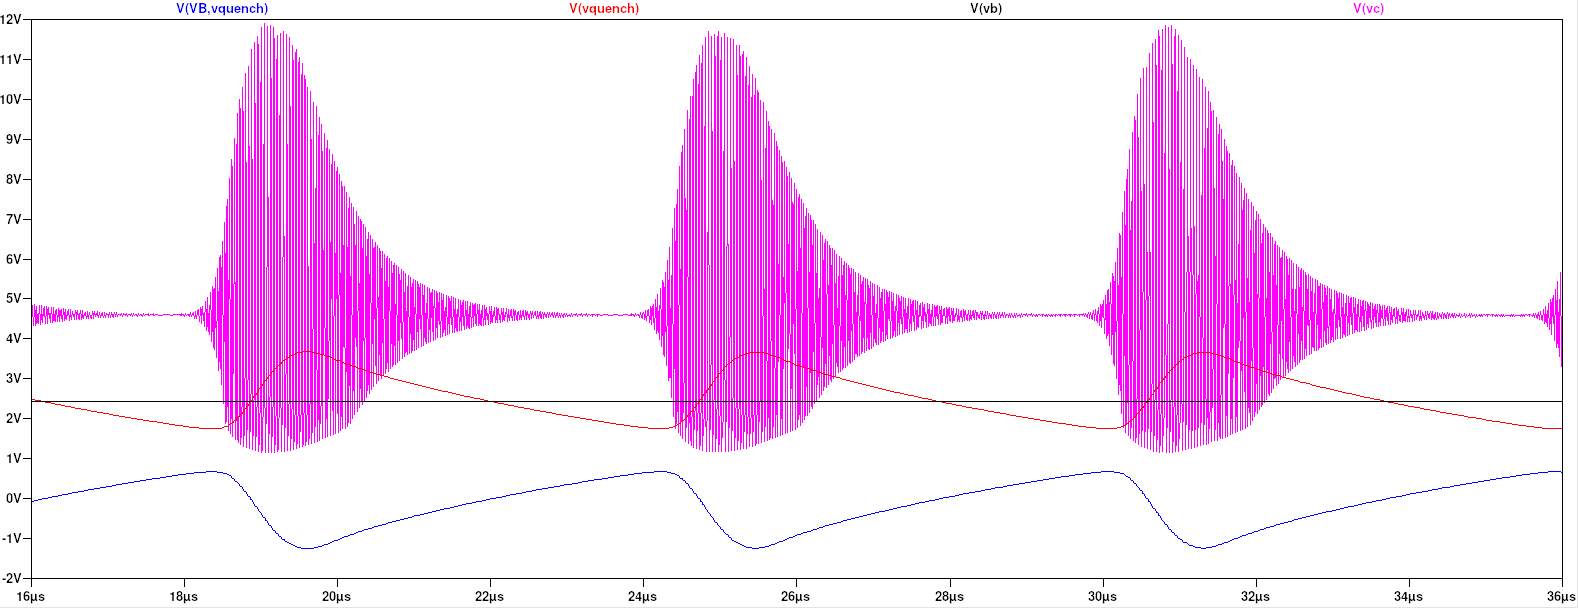
\includegraphics[scale=1, width=1\textwidth]{simrx_zoom}
    \caption{Simulación de puntos de interés en varios ciclos ampliados}
    \label{fig:simrx_zoom}
\end{figure}

\paragraph{Motivos de reemplazo}
Los motivos de remplazo de este modelo fueron varios.
En primer lugar, el sistema de transmisor y receptor no funcionaba a distancias mayores de pocos centímetros. Esto era debido principalmente a la baja potencia radiada. La bobina del circuito tanque de oscilación debía tener numerosas espiras para que a esa frecuencia tan baja consiguiera inducir, por acople magnético, tensión en el receptor.
A parte de el problema mencionado, el transmisor tenía un excesivo consumo estático. En cuanto al receptor, los problemas también fueron varios. Los filtros, tan agudos eran complicados de fabricar, más si los filtros debían ser diseñados a la frecuencia de la portadora como conversión directa. Además, la necesidad de implementar también el demodulador de AM tomando como entrada la señal filtrada se hacía complicado.
Finalmente se opta por mejorar el diseño del sistema proponiendo una segunda versión.

   \subsection{receptor superheterodino FM}
   \paragraph{Desarrollo técnico}
\paragraph{}
Como intento de mejora a la anterior versión, la cual era de conversión directa, se trató de diseñar un receptor superheterodino. A su vez, se mantuvo el diseño del transmisor a varactores, pero se cambió la frecuencia de trabajo a una mayor, unos \SI{6}{\mega\hertz}. 
\paragraph{}
El diseño consistía en un filtro de entrada que era mezclado en un mezclador con un oscilador. Después se realizaba el tratamiento con la señal de frecuencia intermedia. Un amplificador de dos etapas y posteriormente a un rectificador con filtro paso bajo para demodular la señal. Se muestra un esquemático en la figura \ref{fig:crono_sch_receiver_varactor} del receptor sin la parte digital, la cual se explica en el apartado \ref{sec:crono_digital}. La figura \ref{fig:crono_sch_receiver_varactor}, consta de la parte de RF explicada a la derecha, y de la interfaz con la parte digital, un amplificador con realimentaci\'on positiva denominado \textit{Smith-trigger}.

\begin{figure}[h!]
    \centering
    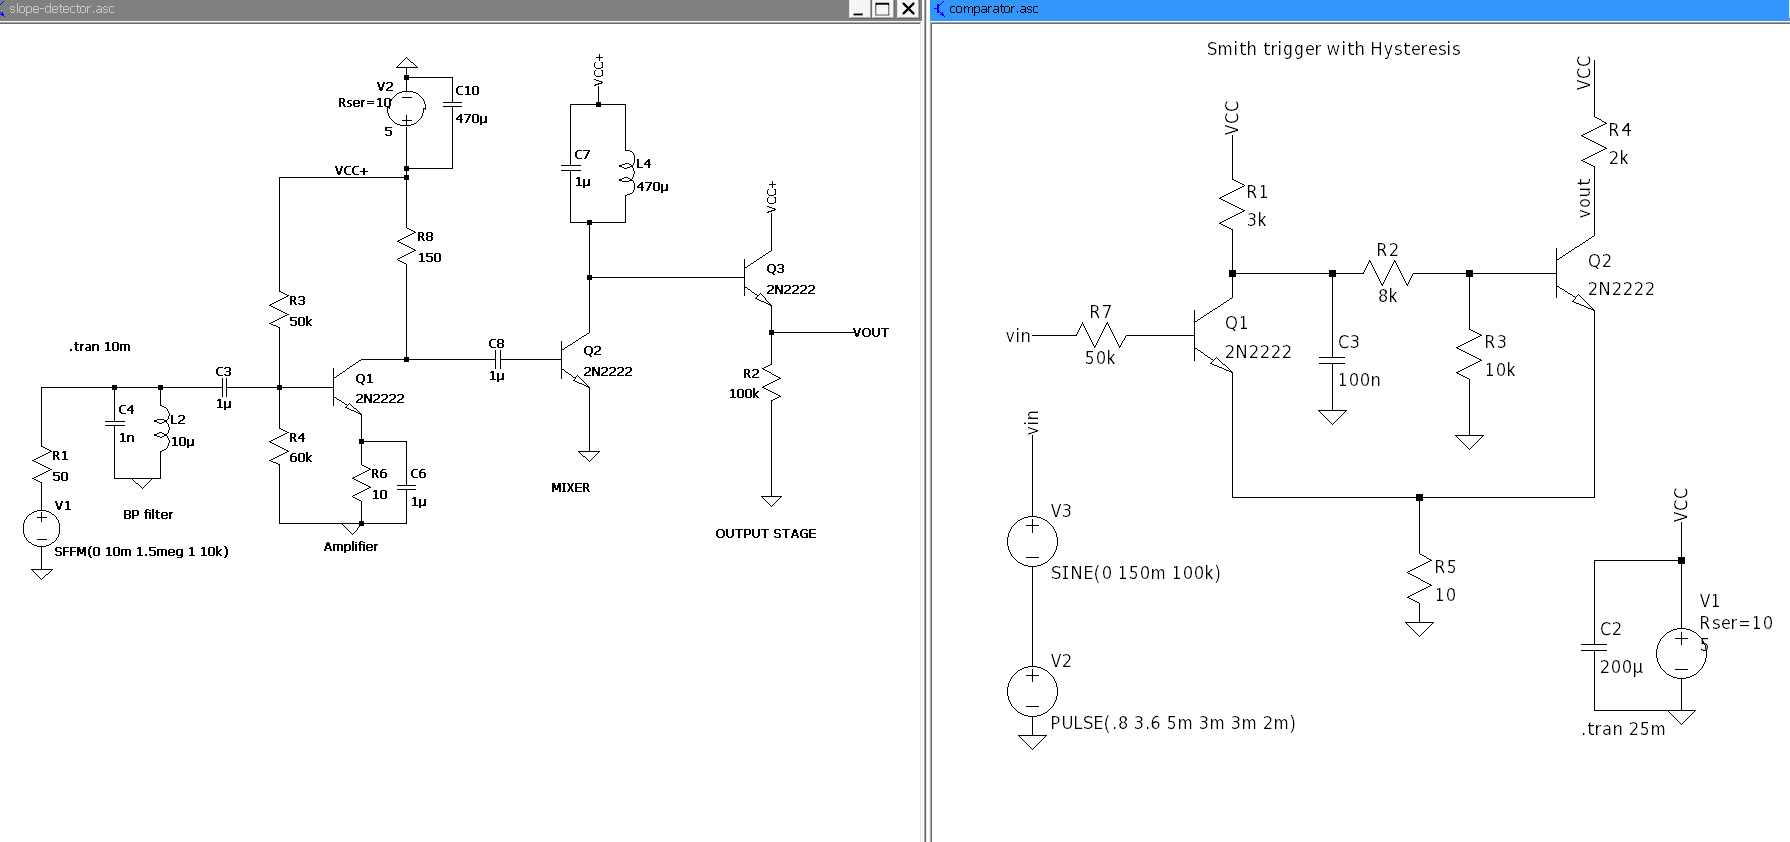
\includegraphics[scale=1, width=1\textwidth]{crono_sch_receiver_varactor}
    \caption{Modelo esquem\'atico del receptor superheterodino de FM}
    \label{fig:crono_sch_receiver_varactor}
\end{figure}

\paragraph{Motivos de reemplazo}
\paragraph{}
Este diseño funcionaba bien cuando se conectaba a la entrada un generador de frecuencias a la frecuencia de trabajo de muy baja potencia.
\paragraph{}
El problema surgía cuando se trataba de probar con el transmisor. 
El receptor no tenía buena selectividad y los amplificadores de frecuencia intermedia, los cuales no estaban correctamente diseñados, producían oscilaciones.
\paragraph{}
Gracias al mezclador, el circuito era capaz de detectar señales de muy baja potencia con muy buena selectividad. A pesar de todo, el mezclador era bastante sensible al ruido, ya que producía bastantes armónicos, producidos por efectos de segundo orden. Esto explica el por qué al conectarlo con el generador, lo más cercano a un tono puro, funcionaba correctamente, sin embargo cuando se trataba de enlazar con la señal del transmisor la cosa cambiaba.
\paragraph{}
También, el diseño general, me parecía que se utilizaban demasiados componentes para unas prestaciones tan bajas. El diseño debía ser sencillo y funcional.
\paragraph{}
Debido a la complejidad a cambio de ninguna clase de beneficio, se opta por transicionar a un esquema de modulaci\'on AM.

   \subsection{M\'aquina de estados digital}
   \label{sec:crono_digital}
   \paragraph{Desarrollo técnico}
El objetivo de este circuito estaba pensado para dar una aplicaci\'on a la señal digital recibida por el receptor. El circuito consistía en una máquina de estados cuya salida tenía una aplicación concreta. En este caso, por cada señal recibida, poner en alto una de sus salidas, manteniendo el estado de las anteriores hasta completar el ciclo, donde todas volverían a estado bajo. 
El esquemático del circuito digital de la máquina de estados se muestra en la figura \ref{fig:crono_logisim}.
Además, se añade en la figura \ref{fig:crono_general}, la integración del receptor superheterodino FM anterior, junto al circuito digital montados en una placa de entrenamiento.

\begin{figure}[h!]
    \centering
    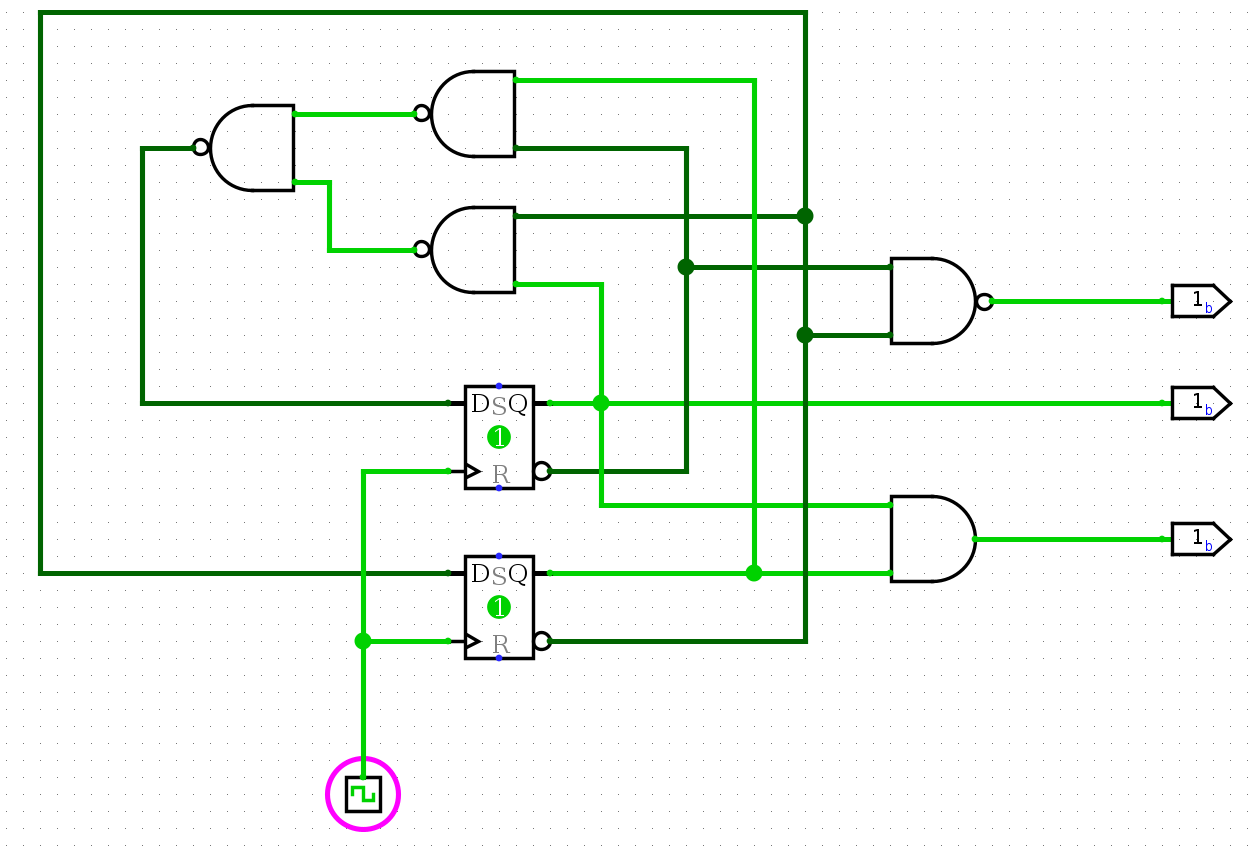
\includegraphics[scale=1, width=.6\textwidth]{crono_logisim}
    \caption{Esquemático de la m\'aquina estados}
    \label{fig:crono_logisim}
\end{figure}

\begin{figure}[h!]
    \centering
    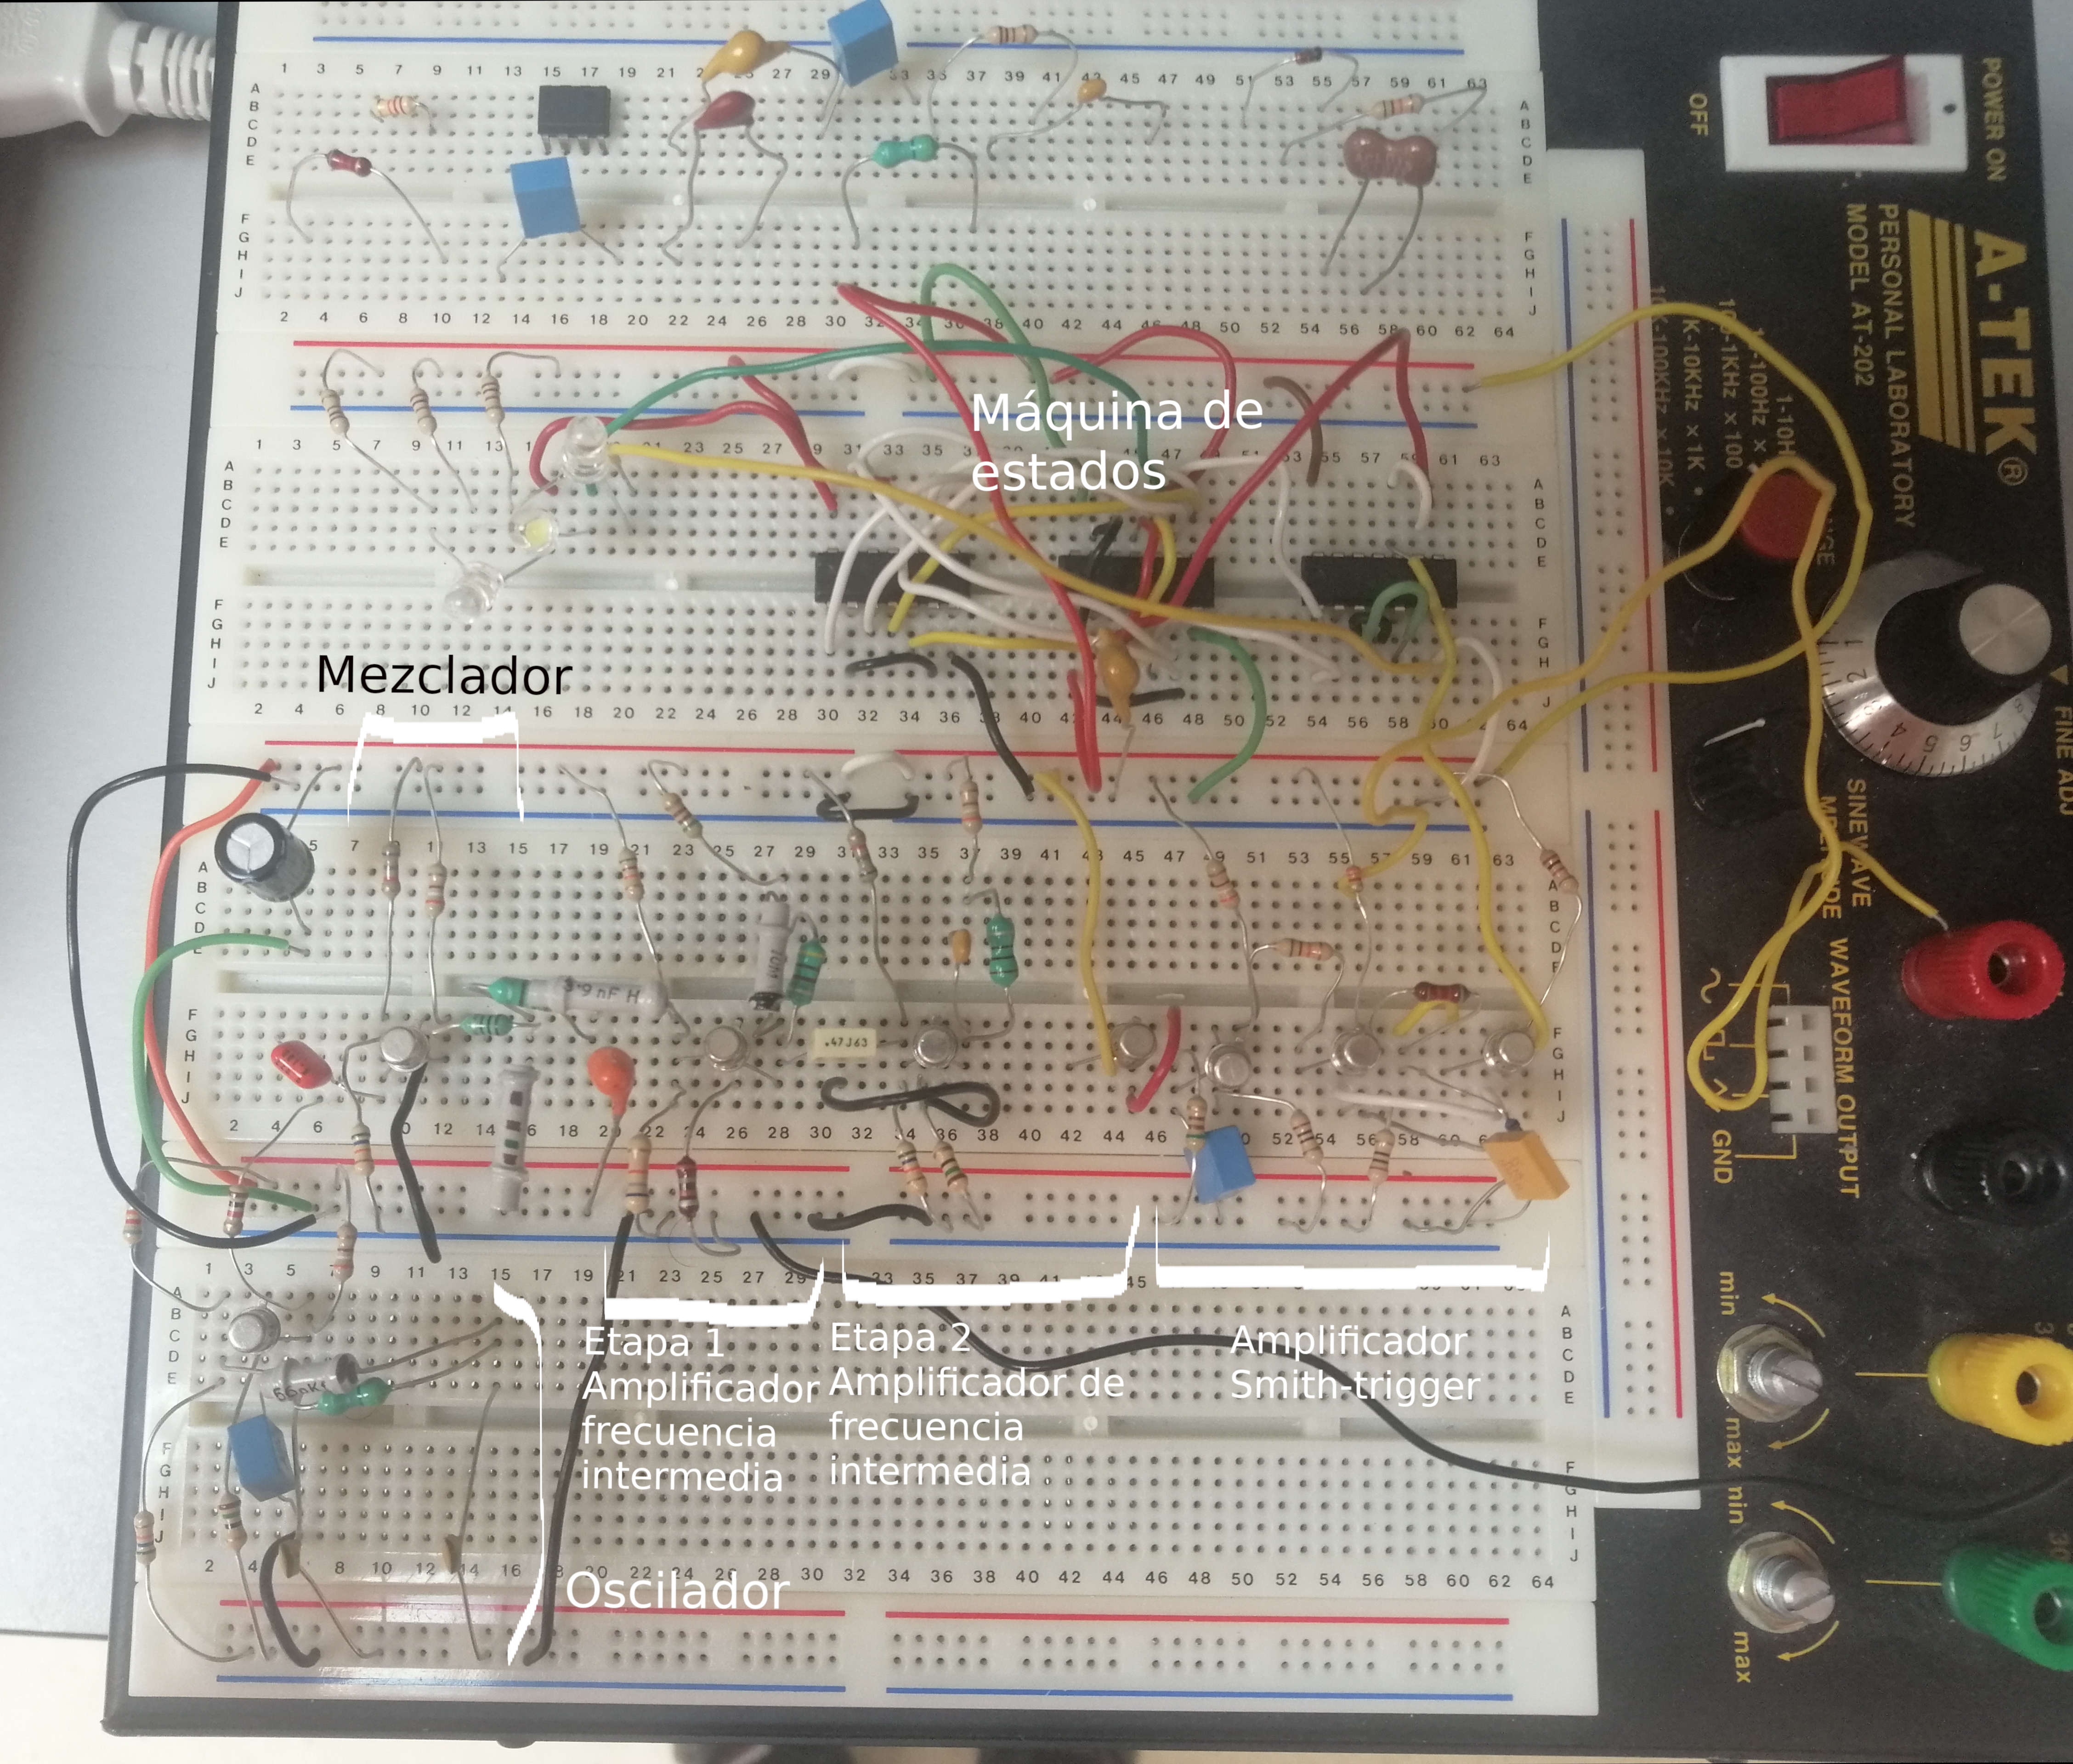
\includegraphics[scale=.7, width=.7\textwidth]{crono_general2}
    \caption{Implementaci\'on del receptor superheterodino de FM completo}
    \label{fig:crono_general}
\end{figure}

\paragraph{Motivos de reemplazo}
El diseño del circuito digital era correcto. Sin embargo, al realizar la integración con el receptor daba muchos problemas debido a que la señal de output del receptor no era fiable. Esta señal, al no estar bien filtrada poseía componentes residuales de alta frecuencia que provocaban que el smith trigger metiera señales falsas. esto provocaba un comportamiento no deseado del circuito. 
\paragraph{}
Para solucionar este hecho, se hizo uso de un microcontrolador. El micro abre una inmensidad de posibilidades como la recepci\'on de múltiples canales, reprogramable en función del uso específico, todo contenido en un menor espacio e incluso con un precio más económico.

   \subsection{Alternativa viable: conversi\'on directa}
   \paragraph{}
posible diseño final funcionaba aunque poca distancia.

   \subsection{Diagrama de Grant}
   En la figura \ref{fig:grant} se muestra el diagrama de Gantt del desarrollo general del proyecto.
\begin{figure}[h]
    \centering
    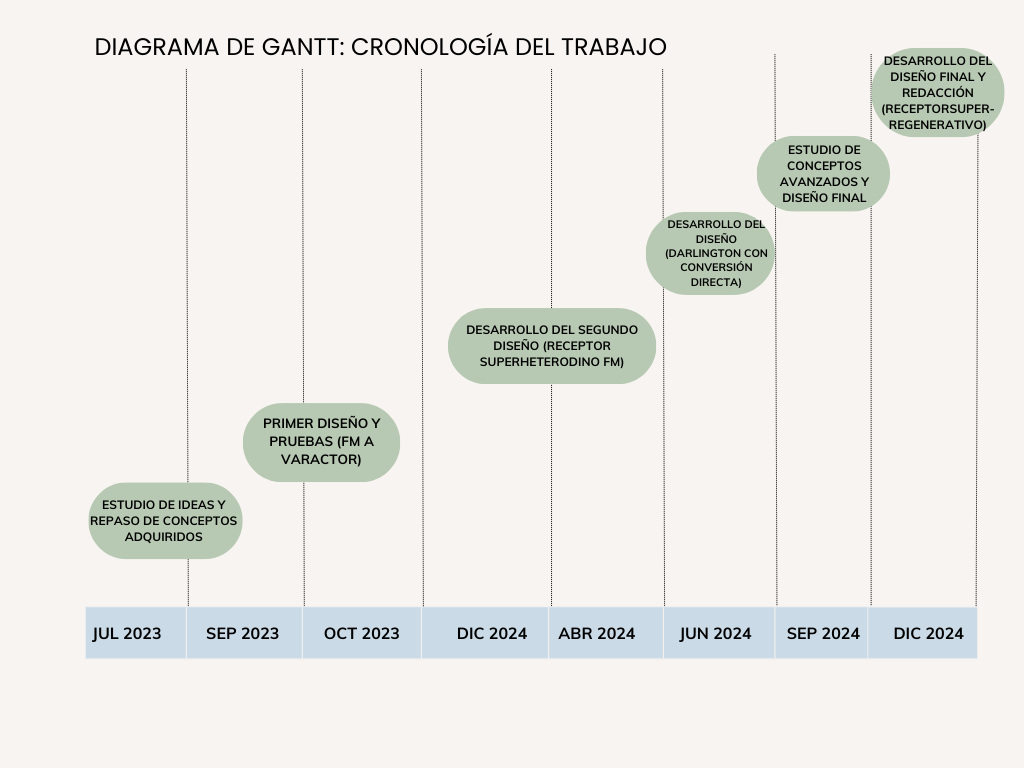
\includegraphics[scale=1, width=1\textwidth]{grant}
    \caption{Diagrama de Gantt del desarrollo del proyecto}
    \label{fig:grant}
\end{figure}

\newpage

\section{Resultados y conclusiones}
   % gestion de ideas y su implementacion en la realidad, diversos niveles de complejidad, un proyecto complicado en la teoria en la practica no funcionaba como se esperaba, al final equilibrio entre complejidad y performance.
% Conocimiento de sistemas de radiofrecuencia y metodos de analisis y visualizacion practica, diversos errores relacionados con RF 
% Relacion de los conocimientos de las distintas ramas que ofrece el grado (control, informatica y diseno digital, fisica y electromagnetismo, radiofrecuencia, electronica analogica).
\paragraph{}
Se concluye con un análisis acerca de si se completaron los objetivos propuestos en el apartado \ref{sec:obj}.
\paragraph{}
En primer lugar, el objetivo de conocimiento de diseño de un sistema de comunicaciones lo considero satisfactorio. Al haber comprendido e interiorizado las bases de los circuitos de radiofrecuencia y puesto en práctica diversas técnicas de recepción de señales de baja potencia como mezcladores, amplificadores o filtros cada uno de ellos diseñado desde cero.
\paragraph{}
Los problemas encontrados fueron múltiples hasta lograr un diseño final. A su vez, fueron múltiples las alternativas propuestas de diferentes desarrollos del sistema. Esto me ha permitido conocer diferentes técnicas de diseño de circuitos de radio. En general, considero satisfactorio este objetivo.
\paragraph{}
En cuanto a la puesta en práctica de los diferentes campos de estudio, considero, en general, que se ha conseguido relacionar los conceptos, por ejemplo, de los lazos de control en conjunto con los modelos de los componentes electrónicos y contrastados con la realidad. 
También, diversos conocimientos de la rama informática a la hora de programar los microcontroladores y establecer todo el entorno de desarrollo. A su vez, se realiza la conexión entre los sistemas analógicos y digitales.
Por último, en el diseño del transformador de la antena englobando toda la parte de radiofrecuencia, antenas y electromagnetismo. Considero satisfactorio este punto.
\paragraph{}
Finalmente, tras tantas posibles alternativas y problemas, se converge hacia un diseño sencillo y funcional con los requisitos tan exigentes que se habían propuesto del diseño desde la raíz. 
Tambi\'en lo considero satisfactorio.

\paragraph{}
En resumen, eval\'uo este proyecto como una experiencia, dura y complicada, que me ha llevado mas tiempo del esperado, pero finalmente satisfactoria. 
De hecho, todos los conocimientos y experiencias adquiridas durante el desarrollo del proyecto, me han permitido lidiar con facilidad numerosos problemas encontrados en mi desempeño a nivel profesional, debido a la asimilacion de numerosos conceptos estudiados en las materias y llevados a la practica.


\section{Bibliografía}
   \paragraph{}
\begin{enumerate}
\item American Radio Relay League (ARRL). (1970). \textit{The Radio Amateur's Handbook}.
\item Franco Peláez, F. J., González Díaz, G., \& Mártil de la Plaza, I. (n.d.). \textit{Apuntes de electrónica analógica}.
\item \textit{Revista Todoelectrónica}. (n.d.). Fascículo segundo.
\item Gray, P. R., Hurst, P. J., Lewis, S. H., \& Meyer, R. G. (2001). \textit{Analysis and Design of Analog Integrated Circuits}. Wiley.
\item González Díaz, G. (n.d.). \textit{Apuntes de electrónica analógica}.
\item Harris, D. M., \& Harris, S. L. (2012). \textit{Digital Design and Computer Architecture}. 
\item Atmel. (n.d.). \textit{ATmega328P Automotive Microcontrollers Datasheet} (Atmel-7810). Recuperado de \url{https://www.microchip.com/wwwproducts/en/ATmega328P}.
\item ON Semiconductor. (2016). \textit{2N2222A: Small Signal Transistor Datasheet}. Recuperado de \url{https://www.onsemi.com/pdf/datasheet/2n2222a-d.pdf}.
\item Kulkarni, S. V., \& Khaparde, S. A. (2004). \textit{Transformer Engineering: Design and Practice}. Indian Institute of Technology, Bombay, Mumbai, India.
\item Horowitz, P., \& Hill, W. (2015). \textit{The Art of Electronics}. Cambridge University Press.
\item {Blake, G. G. (1928). \textit{History of Radio Telegraphy and Telephony}. Chapman \& Hall Limited. Procedencia del original: Universidad de Wisconsin - Madison.}
\item Balanis, C. A. (2005). \textit{Antenna theory: Analysis and design} (Capítulo 4: Linear wire antennas). John Wiley \& Sons, Inc., Hoboken, Nueva Jersey.
\item \textit{AVR Libc User Manual}. (s.f.). Recuperado de https://www.nongnu.org/avr-libc/user-manual/
\item \textit{ArduinoISP}. (s.f.). Recuperado de https://docs.arduino.cc/built-in-examples/arduino-isp/ArduinoISP/
\end{enumerate}


\section{Indice de figuras}
\listoffigures

\end{document}

